\documentclass[11pt]{report}

\parindent 0pt
\parskip 8pt

\usepackage{graphicx}
\usepackage{minibox}
\usepackage{hyperref}
\usepackage{listings}

% reference commands
\newcommand{\fig}[1]{Figure ~\ref{fig:#1}}
\newcommand{\tab}[1]{Figure ~\ref{tab:#1}}
\newcommand{\sect}[1]{Section ~\ref{sec:#1}}

\newcommand{\todo}[1]{\textbf{TODO}:#1}

%Gummi|061|=)
\title{Project CS 2012 Course Report\\Uppsala University\\}
\author{Daniele Bacarella\\
		Jon Borglund\\
		Paolo Boschini\\
		Kiril Goguev\\
		Faroogh Hassan\\
		Marcus Ihlar\\
		Alexander Lindholm\\
		Knut Lorenzen\\
		Harold Mart\'{i}nez\\
		Thomas Nordstr\"om\\
		Thiago Costa Porto\\
		Linus Sunde\\
		Kim-Anh Tran
}

\date{}

\begin{document}

\maketitle



\begin{abstract}
 \begin{abstract}
In Information Centric Networking (ICN), content is delivered to users based on
the name of the requested resource without taking into consideration its physical location.
Based on the NetInf protocol, an Android application backed by an Erlang implementation of a
Name Resolution Service was implemented and both products are presented in this report.
By communicating with each other, the systems store, share and retrieve data objects in an ICN fashion.
In situations of network congestion content is difficult or impossible to retrieve.
Using ICN, the system can provide alternate transfer methods to facilitate the delivering of content.
\end{abstract}

\end{abstract}

\tableofcontents
% ADD LOTS OF REFERENCES HERE!!!!!!!!!!!!!!!!!!!!!!!!!  'multiple exclamation marks are a sure sign of a diseased mind' -- Terry Pratchett
 
\chapter{Introduction}
\chapter{Introduction}

Nowadays the usage of technical devices has become irreplaceable. But with increasing
densification of devices comes network congestion: problems of
browsing the web during a train ride or a concert are apparent. Simply put, the current
location-based networking was not addressed for today's idea of massive content sharing. 
In order to face these problems Information-Centric Networking (ICN) was introduced. For
more information about ICN and all its existing architectures (Data-Oriented Network Architecture (DONA),
Content-Centric Networking (CCN), Publish-Subscribe Internet Routing Paradigm (PSIRP) and Network of Information (NetInf)) 
see \cite{netinf}.
The idea behind ICN is to shift the focus from hosts that serve a content to the actual objects that
are shared. More specifically, these Named Data Objects (NDO) shall no longer be coupled
to a host that is owning the content, but shall ideally be retrievable from \textit{anywhere}.

This report picks a proof-of-concept implementation of the usage of NetInf
(see \sect{netinf}), one out of four concepts that realize ICN. The software was
developed in the context of the 
\textit{Project Computer Science}\footnote{\url{http://www.it.uu.se/edu/course/homepage/projektDV/ht12}},
a course under the supervision of Olle G\"{a}llmo and in cooperation with Ericsson Research \cite{ericsson}
in 2012/2013. The goals set for this project are listed in \sect{goals}. 

The product itself consists of two separate parts developed by two development teams within the same project group. One is an Erlang \cite{erlang} implementation of a Name Resolution Service (NRS) with streaming capabilities.
The other product is a browser application called "Elephant" for Android \cite{android}  phones that takes advantage of NetInf services that
are based on OpenNetInf \cite{opennetinf}, an open source Java implementation of NetInf. 

Both products are described more in detail in \sect{product}. For a thorough understanding
of the implementation and extension of the current state, preliminaries and system architecture decisions are 
described in \sect{preliminaries} and \sect{architecture}. 
The performance of both products are evaluated in \sect{evaluation} and based on the results,
\sect{conclusions} discusses the future work and draws conclusions for the developed products. Finally, the appendix contains installation as well as maintenance instructions.

\chapter{Resources}


\section{Project Group}

\begin{table}
\centering
\begin{tabular}{|l|c|}
\hline
Group member & Nationality \\ \hline\hline
Daniele Bacarella & 
\includegraphics{graphics/it.png} \\
Jon Borglund & 
\includegraphics{graphics/se.png} \\
Paolo Boschini & 
\includegraphics{graphics/it.png} \\
Kiril Goguev & 
\includegraphics{graphics/bg.png} \\
Faroogh Hassan & 
\includegraphics{graphics/pk.png} \\
Marcus Ihlar & 
\includegraphics{graphics/se.png} \\
Alexander Lindholm & 
\includegraphics{graphics/se.png} \\
Knut Lorenzen & 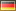
\includegraphics{graphics/de.png} \\
Harold Mart\'{i}nez & 
\includegraphics{graphics/ve.png} \\
Thomas Nordstr\"om & 
\includegraphics{graphics/se.png} \\
Thiago Costa Porto & 
\includegraphics{graphics/br.png} \\
Linus Sunde & 
\includegraphics{graphics/se.png} \\
Kim-Anh Tran & 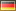
\includegraphics{graphics/de.png} \\
\hline
\end{tabular}
\caption{Each group member's nationality}\label{fig:nationality}
\end{table}

In our project we are 13 students coming from 7 different countries (see \fig{nationality}).
It was a great experience to have team mates from different parts of the globe - not
only working-wise but also food-wise! As our fika rule states, any person who comes later
than 9 o'clock should bring fika for the rest of the group. Thus, we could
try Teque\~{n}os ("cheese sticks") from Venezuela or Tiramisu from Italy.\\

Due the scale of the project, the group decided to divide into two teams. 
The frontend team (LISA), responsible for implementing the client side of the NetInf project and the backend team (ERNI), responsible for implementing the server technology.\\

The groups were divided as follows:

\begin{minipage}[b]{0.32\hsize}\centering
\begin{tabular}{l}
The Frontend team (LISA) \\\hline
Paolo Boschini\\
Harlold Martinez\\
Thiago Costa Porto\\
Linus Sunde\\
Kim-Anh Tran
\end{tabular}
\end{minipage}
\hfill
\begin{minipage}[b]{0.32\hsize}\centering
\begin{tabular}{l}
The Backend team (ERNI) \\\hline
Daniele Bacarella\\
Jon Borglund\\
Kiril Goguev\\
Faroogh Hassan\\
Alexander Lindholm\\
Knut Lorenzen\\
Thomas Nordstr\"om
\end{tabular}
\end{minipage}

Since we had two office rooms, each team could have one of its own.
Nevertheless, we needed to continuously communicate with each other,
since we were working on the same project with the same customer.

\subsection{Seating arrangements}
The seating arrangement of both groups are shown in \fig{frontend_seating} and
\fig {backend_seating}. The main point of the seating within both groups
was to face each other, so that social interaction and communication was facilitated. 

For bigger discussions though, the backend team used the coffee room, whereas the
frontend team had a separate discussion table in the corner of the room. Therefore
other team mates could continue working without being distracted.

\begin{figure}
\centering
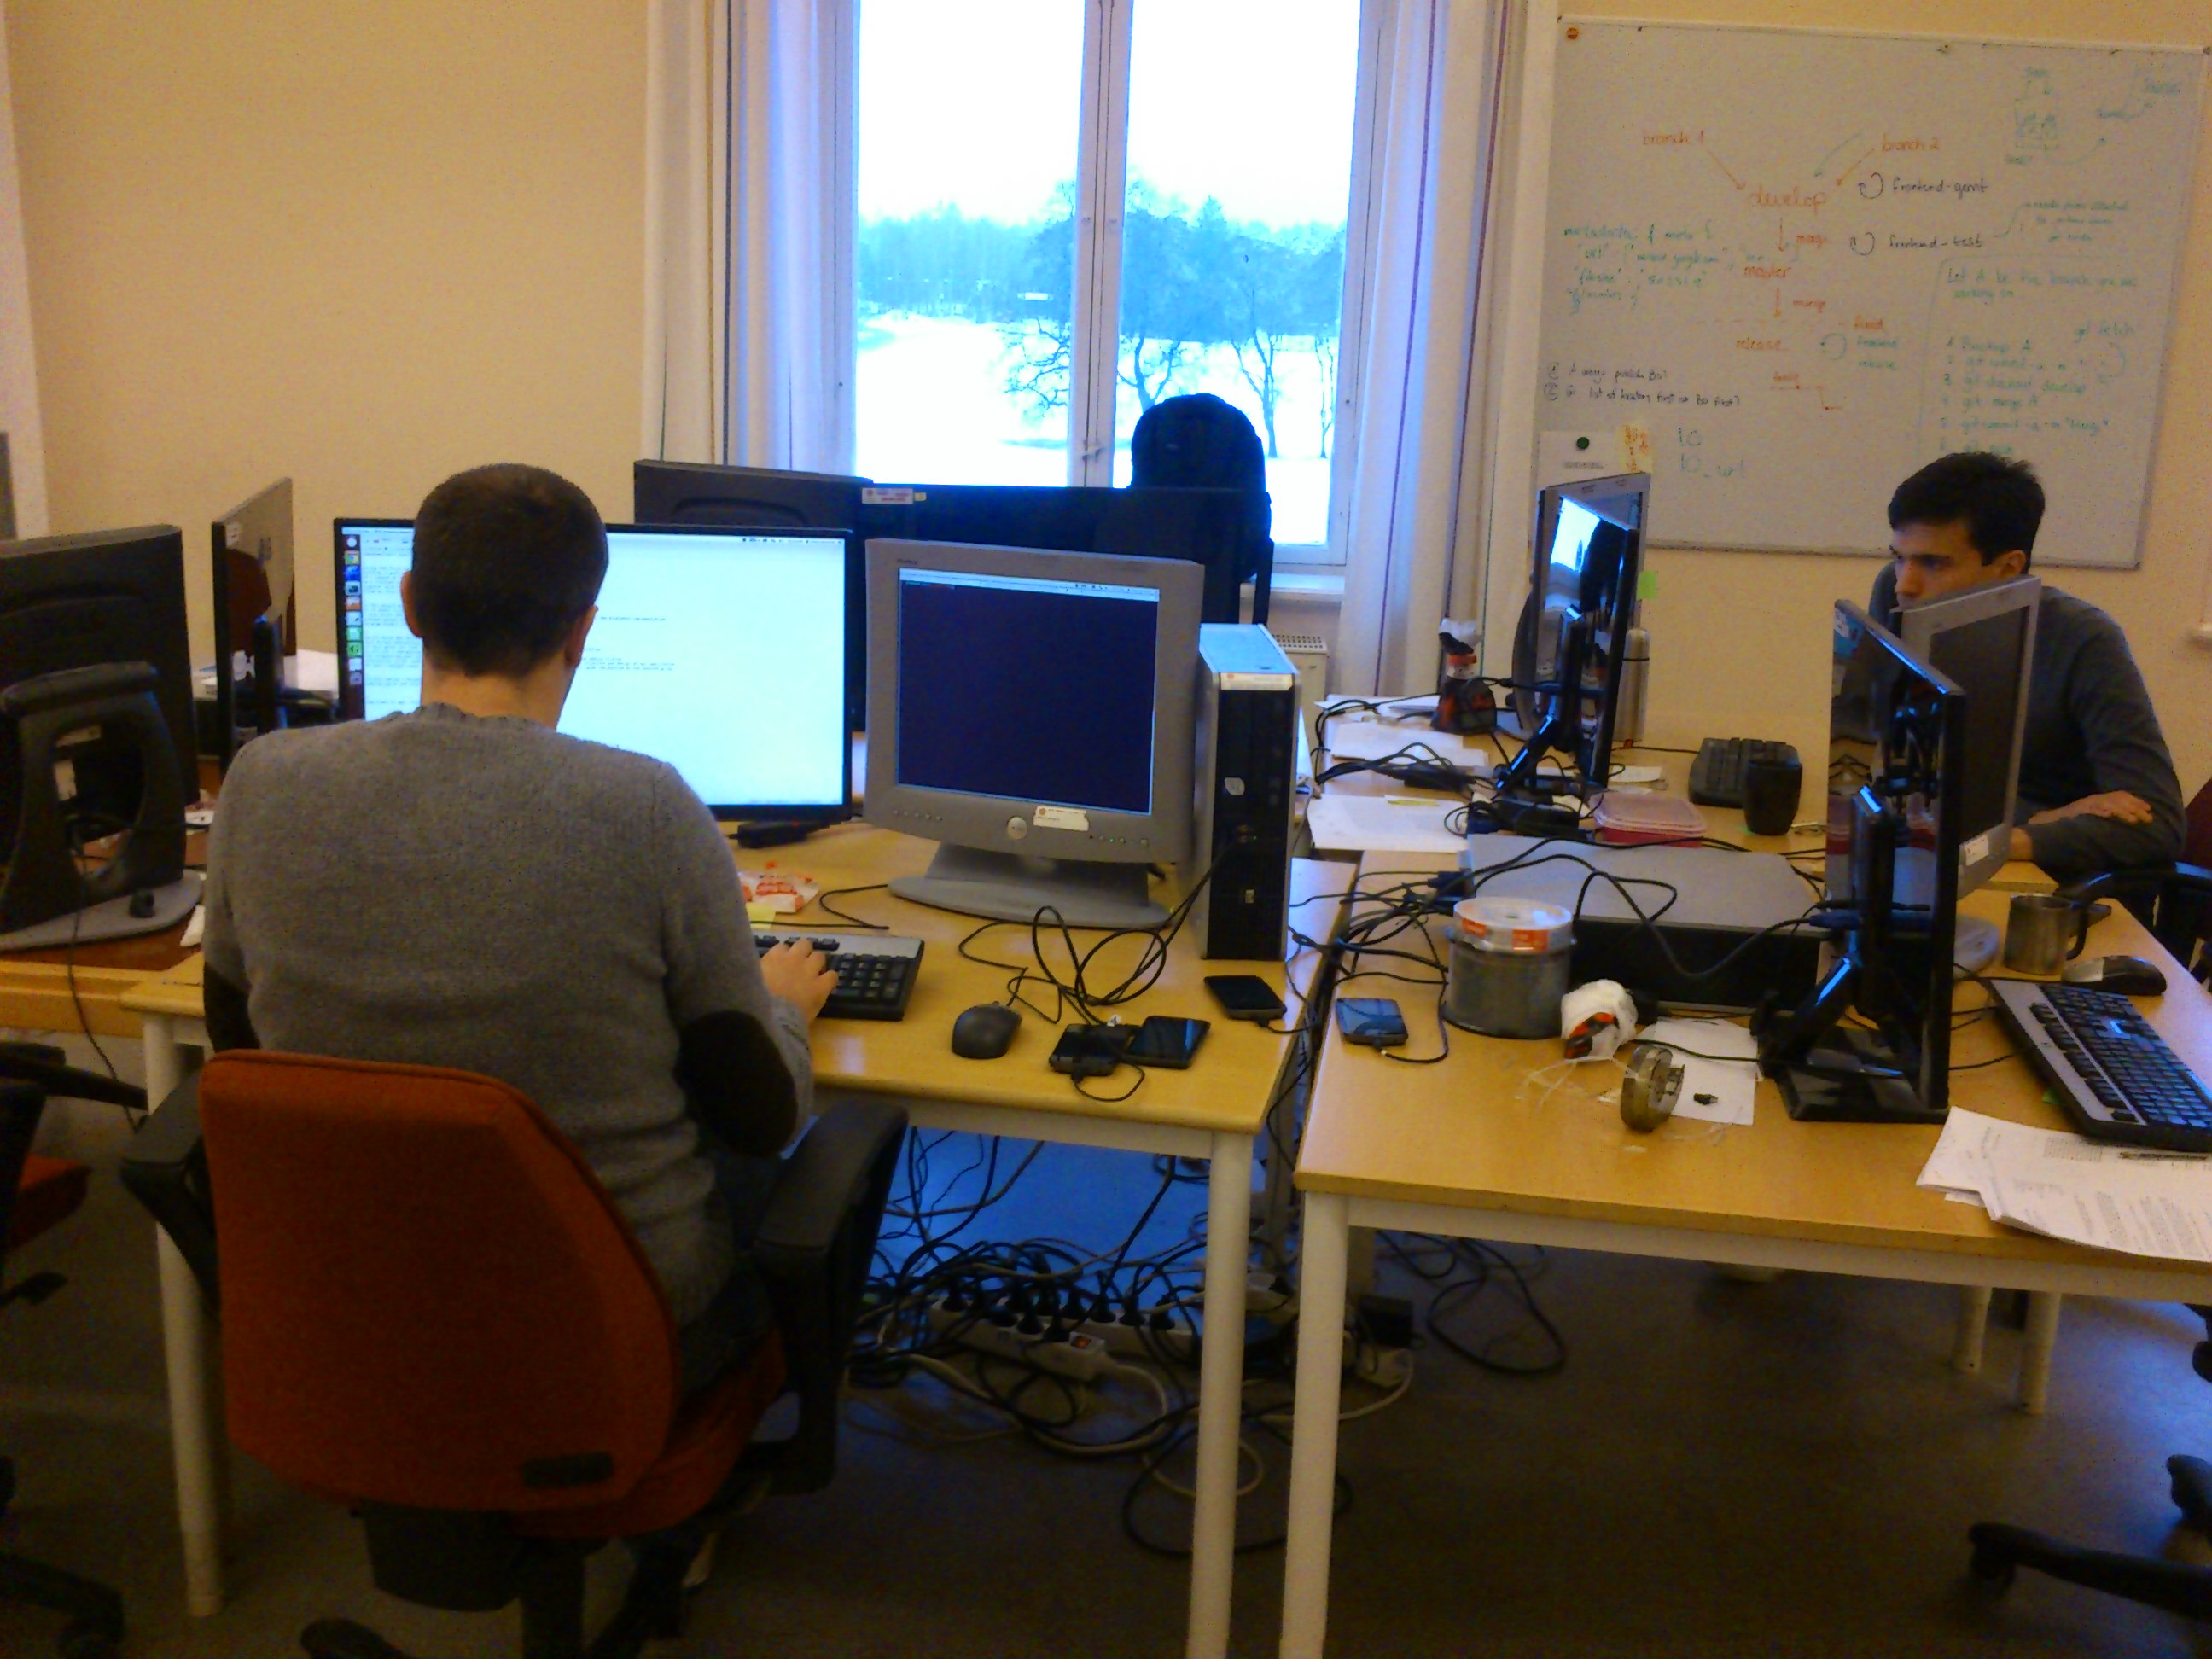
\includegraphics[scale=0.1]{graphics/frontend_seating}
\caption{Frontend seating arrangement}\label{fig:frontend_seating}
\end{figure}


\begin{figure}
\centering
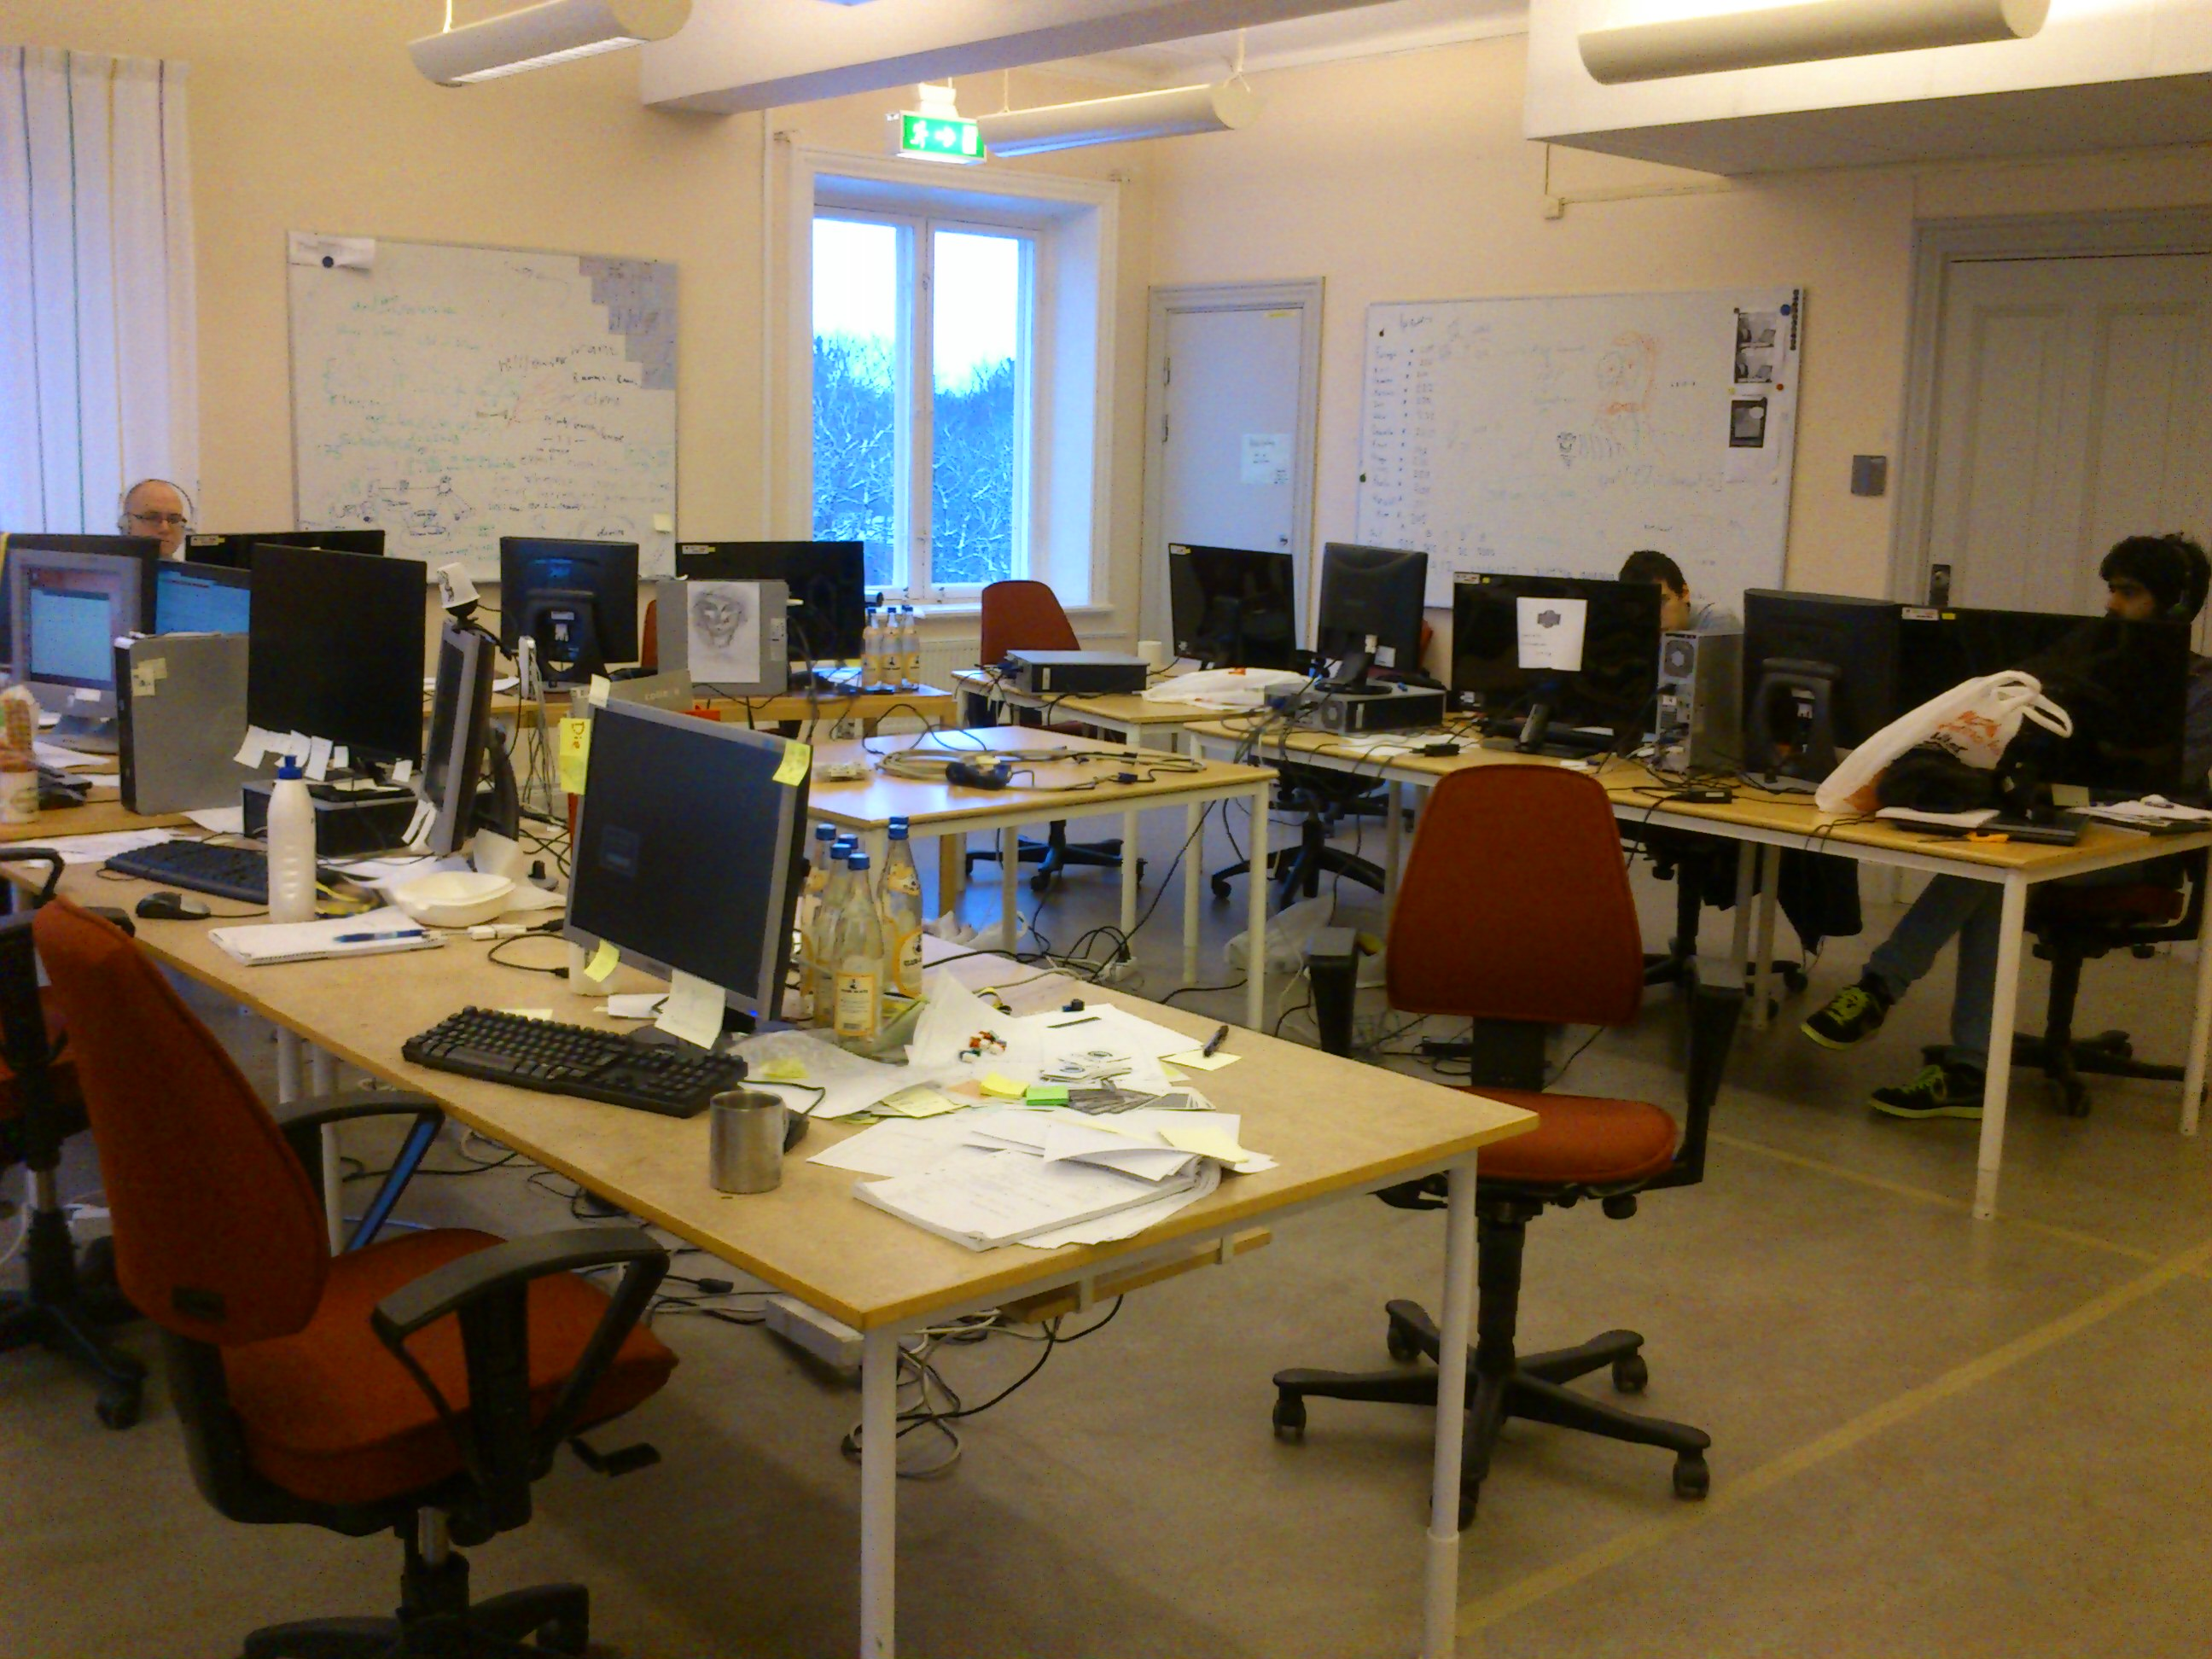
\includegraphics[scale=0.1]{graphics/backend_seating}
\caption{Backend seating arrangement}\label{fig:backend_seating}
\end{figure}

\section{Equipment}

All the members in the teams were provided with a Desktop PC. In addition to the main development PC's there was three servers running Git, Redmine, JIRA and Jenkins and a projector from Uppsala University. The teams installed Ubuntu 12.04 LTS on all the machines.

Ericsson Research also gave the LISA team eight android phones for development and testing. Each Android phone came with the JellyBean Android OS. 






\section{Tools}
\label{sec:tools}
\subsection{Development Languages}

The LISA team used Android - Java based development language. Their application was targeted at JellyBean Android OS version 1.4.1(Version 16).

The ERNI team used Erlang, Javascript, HTML 5  as their development languages. The main product was coded in Erlang. During the final sprints the client wanted to add video streaming. As a result of this ERNI also created a html client interface to our system using Javascript and HTML 5. 
\subsection{Continuous Integration \& Build Server}

We adopted a continuous integration server which allowed the developers to create special 'jobs' which will control the compilation, error reporting/blaming and source control. Other instances of this project used tools like buildbot but after a long and fruitless effort to make and configure buildbot properly we determined that buildbot was a waste of time and looked into a more powerful/user friendly CI server called JENKINS. 

Jenkins is a CI server with a HTTP interface that allows you setup custom jobs for your project. Things like monitoring a version control system for changes or running command line arguments on the code in your project is easy and user friendly with plenty of tutorials and resources online. We used Jenkins to control both the ERNI and LISA project. 

Jenkins was particularly useful for blaming individuals who 'broke the build'. If Jenkins is configured with the email addresses of all people and a build job fails after someone has updated the source code then, Jenkins will send an email out notifying those who have broken the build and those who are affected(all other collaborators on the current code file which is broken).

We have generated a document which explains how to setup and use Jenkins as we have done in this project. 
\subsection{Version Control}
\label{sec:git}

In order to keep the workflow going at a good pace the teams elected to have version control, which is good practice in all projects. Git was used with a custom workflow shown below. \\

Have a server side repository with 4 initial persistent branches.
\begin{itemize}
\item master
\item staging
\item develop
\item release
\end{itemize}

The following naming convention for temporary branches is adopted: 

\begin{itemize}
\item SprintX.shortStoryName
\end{itemize}

NOTE: The temporary branches will be deleted after each successful merge to the DEVELOP branch.

\subsection {Policies}
\begin{itemize}
\item master\\ \\
The 'master' branch will only contain Demo code. This is the code which contains ONLY the fully tested and integrated stories.  \\\\Tags will be made here under the following convention:\\ \emph{SprintX.shortStoryName} \\\\
This is a Jenkins build tool controlled area - No human user should be operating in this branch. \\Jenkins is responsible for  merging from 'release' to 'master' at the end of a sprint- in order to keep the branches synchronized and provide a fresh clean start for each sprint from working demo code.\\
\item release\\ \\
The 'release' branch will only contain individual stories which are completed and fully unit tested. Here the team can pick and choose which stories to include in a specific demo. This branch is also a Jenkins build tool area. \\Jenkins is responsible for integration testing and merging between 'release' and 'master'
\item develop\\ \\
The 'develop' branch will contain all the code that is able to be compiled on the server and is where the human users will start their personal story branches. Also a Jenkins build tool area, the code here will be considered in a "Story done and compiles but not yet tested" state.\\ Jenkins is responsible for unit testing and merging between 'develop' and 'release'

\item staging \\ \\
The 'staging' branch will contain all the dirty code and is where the human users will push code when finished at the end of the day. Also a Jenkins Build tool area, the code here will be considered as a story is in progress it may be done but it also may not compile. Jenkins will pull all the code from this branch and try to compile it, if it compiles then it will be merged with the 'develop' branch.

\item SprintX.shortStoryName\\ \\
The branch's name will contain the local working code for the specific sprint story followed by a short story name-typically the name written on the post it note for example: Message\_Handler. A merge to the 'develop' branch will mean the story is considered done for the sprint but requires testing by integration tools and Jenkins. This branch will be deleted after the tests are passed and the a successful merge is complete.
\end{itemize}

For instructions on how to utilize this workflow see Appendix B \ref{gitworkflow}.

\section{Project Management}

There have been many suggestions from previous instances of this course to use project management/issue trackers. Initially both teams were using Redmine\cite{redminesite} but then decided to diverge and try out another project management tool. 

\subsection{Redmine}

The ERNI team decided to use Redmine\cite{redminesite} for the duration of the project. The tool provided useful features such as
\begin{itemize}
\item Wiki
\item Version Control explorer
\item Bug and Issue tracking
\item Time keeping
\item File storage
\end{itemize} 

Redmine is easy to install and free of cost, including plenty of plugins for various needs. BitNami offers a free one-click-installer package for Redmine. Both teams started the first sprint with Redmine installed and two projects configured. Redmine was used heavily for the first sprint by ERNI for creating issues and trying to keep track of time spent for each task in order to aid in planning the time required for each task. 

However by sprint two's retrospective and a changeover to a new Scrum master, the ERNI team decided to drop the issue tracking and the time keeping as they felt it was too much overhead and did not help so much with the time estimation of tasks. The wiki became the most extensively used feature of this tool followed by the Version control explorer. 

Instead of creating issues and assigning them in Redmine the ERNI team opted for a simpler solution, writing tasks on post-it notes and adding them to the Scrum board. Even though this was simpler, it became messier as sprints became longer.

\subsection{JIRA}

The LISA team wanted to test out JIRA\cite{jirasite} since they had many issues getting the plugins and the right functionality for their team. JIRA unlike Redmine is not free, and comes with a 3 month trial license. LISA felt that this provided much more functionality than Redmine and was easily customizable.

JIRA worked well for LISA as each member was at one point Scrum Master, and was able to keep work logs, issues and assign tasks easily. The major point for using JIRA was persistence as each Scrum sprint was catalogued.

\chapter{Project methodology and organization}
\section{Scrum}
\label{sec:scrum}
Scrum is an agile software development framework that is used for planning, managing
and undertaking a software project. Scrum is designed to optimize flexibility and productivity,
as it demands short working phases (sprints) that make it possible to deliver
a working software product continuously throughout the project. Thus, the Scrum team
can react on time when the customer changes the product specifications.

Agile methodologies are rapidly becoming the standard
in software development companies. As a student, the Project CS is a great opportunity
to experience Scrum, as we are about to go into the real world of software development.

\subsection{Roles}

Scrum distinguishes between the Scrum Master, the Product Owner and the Development Team.

The Scrum Master acts as a bridge between the team and the product owner. 
He is responsible for making sure that the team adhere to the Scrum guidelines. He is not to be seen as the head of the group, but instead as someone who's main responsibility is to remove impediments in completing a task.
He should also make sure that the team is on the right track keeping a constant eye on the sprint goal
and the definition of "done" for the different tasks. On the other hand, the Scrum Master
needs to ensure that nothing interferes with the development team so that the developers
can constantly concentrate on their work.

The Product Owner is an individual who can be seen as a connection between the client and
the development team. Within the team, the Product Owner acts as the client, although the client normally is an external actor.
The Product Owner is the person who owns and controls the development of the software with the help of the backlog,
prioritizing features and generally the one who is supposed to give direction to the devlopment team during the sprint planning and at the product demonstrations.
In some cases, the Product Owner can be the same person as the client.

The Development Team is the set of individuals who are working on the project for the product owner.
The team is responsible for creating increments and releasing a working version of the software
after each sprint.


\subsection{Scrum Keywords}
\begin{itemize}
\item{\textbf{User story}}\\
A user story is a description of an end user interacting with one small part
of the product. It gives the developers an intuition of what functionalities need to be available
to accomplish the intention of the user.
Each product requirement is translated into a user story. Stories are usually
broken down into tasks and each task is the smallest unit of work to be implemented.
It is important that the development team agrees on the definition of "done" for each task and story.

\item{\textbf{Product backlog}}\\
The product backlog is the ordered list of all user stories for a product. The backlog
is created by the customer.
Stories are prioritized by the product owner depending on criteria such as date needed or business value.

\item{\textbf{Sprint}}\\
A sprint is the core artifact of Scrum. A sprint is an iteration that usually lasts between two to four weeks
during which a part of an entire product is implemented. Each sprint has a goal and each member of
the team should strive to fullfill that goal. The whole project period consists of several sprints.

\item{\textbf{Sprint planning}}\\
In the beginning of each sprint the team meets for planning and agreeing on the current sprint's goal.
Stories are picked from the product backlog and broken down into tasks. The team estimates the workload
for each task and moves the highest prioritized tasks from the product backlog to the
sprint backlog. This is done until the maximum workload is reached for the sprint. The output of the sprint planning
is a sprint backlog that everyone agrees on. 

\item{\textbf{Sprint backlog}}\\
A list of stories that should be completed by the end of the sprint. The sprint backlog is filled by picking the highest 
prioritized stories one by one from the product backlog. 

\item{\textbf{Sprint demo}}\\
At the end of each sprint a demo is scheduled with the client. At the demo the team presents the results of the sprint 
in the form of a working product to the customer. The good part of having frequent demos is that the team and the customer can
feel the progress. It is also an opportunity to see if the customer and developers share the same idea.

\item{\textbf{Sprint retrospective}}\\
After each sprint is completed, the team gathers together to reflect on the good and bad parts of the sprint.
To make improvements throughout the project it is important that everyone is honest and shares their opinion during the retrospective.
This is the point where you can not only improve the working process but also the team environment.

\item{\textbf{Standup meetings}}\\
A mandatory short meeting (usually 10 minutes) starting every day at the same time.
Each person tells the others what he did the day before and what he is going to do
next. The participants attend the meeting standing up so that everyone is encouraged to be concise
when telling the status of their work.

\end{itemize}
\pagebreak

\subsection{Scrum process}
The following picture summarizes the Scrum methodology.

\begin{figure}[!h]
\centering
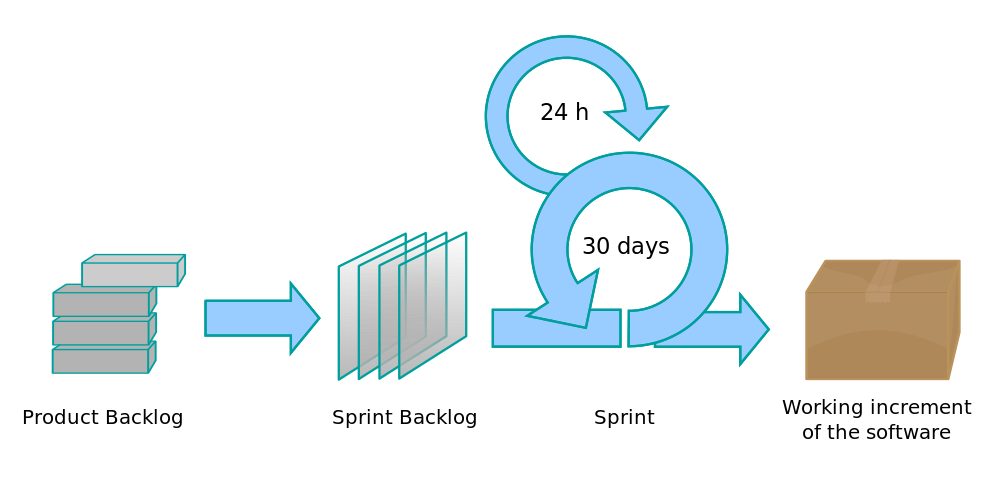
\includegraphics[scale=0.35]{graphics/scrum.png}
\caption{The Scrum Process}\label{fig:scrum_process}
\end{figure}

\section{Use of Scrum in this project}
Throughout the project the teams tried to apply the Scrum methodologies thoroughly.
Both rooms and desks were arranged to facilitate direct communication among team mates, as well as setting up a whiteboard for the post-its. 
The frontend team agreed that each team member should try to
be the Scrum Master at least once during the whole duration of the project.
Project CS provides a great advantage in that it is a course within university and the Scrum master role could easily be shifted from one person to the next..
Since there were two teams, there was always two Scrum Masters, one for each team.

\subsection{Daily meetings}
Due to the separation of the group into two teams, there was two distinct sets of meetings in the offices.
Daily meetings for the frontend team took place everyday at 9:00 o'clock sharp and time boxed to 15 minutes,
while at 9:15 the standup meeting would start for the backend group.
Both scrum masters were present at each meeting.
The reason for this was to facilitate synchronization between both teams.

In our opinion these meetings were of great value. 
They encouraged everyone to actively talk to the other team members about
the status and their problems.
Each stand up meeting was mandatory so that we could be sure
that everyone would start working at the time. 
Moreover it was a good way for planning short tasks and catching bad decisions early.

\subsection{Sprint planning}
After each demo the teams planned the sprint for the next iteration, trying to get done before the weekend.
In this way work started directly at the beginning of the new week. Most of the times the demos were on Thursdays. Thursday was chosen so that pre-planning could be done on the same day and meet the client on Friday for planning approval.

To estimate of the available working days for each sprint, the teams calculated the total amount of days
according to the number of the team members, and used a productivity factor of 0.7. One story point corresponds to one man day (8 hours). A team of 5 developers working
for two weeks would have 5*10*0.7 = 35 available story points.
In order to estimate the workload of each story planning poker was used. Each individual had a set of cards
with numbers and votes with a card giving points to each story. 

In our case, the requirements were not set from the beginning. Therefore the teams had a continuously
changing product backlog, which was updated at each pre-planning phase.

\subsection{Demo}
Demos were held at the end of each sprint during which the teams showed their results.
We demonstrated the application to Olle, Muneeb and Ericsson in a very relaxed environment. Having short sprints and doing frequent
demos ensured that Ericsson saw progress often.

\subsection{Retrospectives}
Retrospectives were done in form of meetings after each sprint. Each member had to say three good things and three bad things about
the completed sprint. It was a great way to point out what was positive during the sprint
and to expose constructive critics for the bad parts. In this way the teams could always try to improve the process in the next sprint.

\subsection{Conflicts}
In any large group project there will be many different personalities, opinions, experiences and backgrounds. Some people have very little experience of working in larger groups(10+ people). This course forces the members to work together and to do it in a specific project management style(Scrum). It is inevitable that there will be conflicts and disagreements. 

The following are some points that the teams followed when there were conflicts.
\begin{itemize}
\item Try to address the problem with the individuals involved together.\\ \\
The first and foremost approach is to try to talk it out with the people involved. Please note that you may have very different personal and work experiences. This is a good thing but keep in mind that how you worked in a previous course or at a previous workplace may not be the best way to do it in the current project. It is best to come to the project with an open mind and offer your past experiences as a way to suggest how to go about preforming certain tasks, but never blatantly ignore everyone else because you feel they are wrong. This course is a team-effort based project and not to be treated as a workplace, here you are allowed and even encouraged to make mistakes and to learn from them.

\item Realize that just because you do a task does not mean that it was the right one.\\ \\
The idea of Scrum, simply put, is to change the product during the development cycle quickly. As developers we may sometimes get attached to the code we have written and can take offence when the team or client decides to remove the code. In this case it is not a matter of the team or client attacking you, it is a matter of whether or not the code or task is still relevant to the project after a design change. The project will be very different from the beginning to the end. Code will be obsolete and deprecated at certain points, just live with it and continue contributing and understand that your work is still recognized by everyone else.
 \\
\item Use the Scrum master as a mediator.\\ \\
In the case where addressing the problem yourself did not work out, the use of Scrum in this project gives everyone a great resource, the Scrum Master. It is the Scrum Masters duty to remove impediments in the sprint, however big or small. Conflicts are a great impediment and can sometimes lead to failed sprints and worse, de-motivation of the team. The Scrum Master should in this case act as an impartial mediator. And strive to come up with a solution to the problem, even if it means making sure the conflicting personalities do not work together in the end if it can be avoided.

\end{itemize}

\section {Quality Assurance}
In large projects you need to be able to control the quality of your product. Does it do what the customer asked? Is it extensible? Is it releasable? While some companies have specific quality assurance teams, this  course usually does not. Therefore, the team had to explore ways of answering the above questions.

While SCRUM and Agile methodology easily answers the ``Is it releasable?'' question, just because you implement SCRUM and Agile does not mean you are doing it correctly. In SCRUM, at the end of every sprint you should have something that is demo-able. Sometimes this is not the case -- failed sprints, outstanding issues, etc.

\subsection{Pair-programming}

Both teams decided to take the pair programming approach to quality assurance. Two programmers complete a task and two other programmers review that work for bugs, imperfections (according to code standards), and integration status. 

The ERNI team felt that this worked particularly well as we all had little to no experience in functional programming and large group work projects. Often bugs were caught way before the task was completed and put into the review process. 

Using pair programming also helped develop our skills faster as we taught each other how the language worked and had knowledge redundancy (if one person was away the task would not be stopped). After review you had twice as many members of the team having full knowledge of the code and functionality introduced into the product.

\subsection{Code Reviews}

The LISA team decided to use a tool called \textit{Gerrit} to preform code reviews. Gerrit is a web-based code review system, which makes it easier for us to do the review, as every team member can see what is up for review and what has been reviewed at all times. Gerrit is dependent on Git and acts almost like a filter, only allowing authorized changes to be pushed to the master branch on Git. Therefore, it promotes code quality by forcing code reviews to take place before code is placed on the repository.

Initially, we had some trouble setting up the tool. While installing Gerrit itself is not a problem, integrating it with Jenkins was a bit of an issue. After a few emails with the maker of the Gerrit/Jenkins plugin, we found out that the issue was due to encoding in the terminal. Make sure you have the proper terminal encoding (UTF-8) before setting it up. After this small mix-up, Gerrit was ready to be used and tests suggested that it was working properly.

After everything was running, it took us about 2 hours to drop Gerrit altogether. The reason for it was mainly cultural -- we implemented a code reviewing tool in the middle of the project -- and we did not have enough time at that point to invest in learning how to do it properly and maybe circumvent the main issue we had with the tool. The main issue was that, in our team of 5, code was flying around back and forth. New feature branches was created and merged into the main branch. These branches often contained features that was required by other features that were being developed at the same time. Gerrit provided a filter, as advertised, but it ended up with not being very productive for us. We would have to change our workflow and, in the middle of the project, that was a major overhead for all of us. Being a team of 5 people, we could manage, to a certain degree, the code quality by doing pair programming and reporting to others about strange code that one has come across.

Gerrit is a very nice and interesting tool, which will probably help your development a lot \emph{if} you implement it before the actual coding has begun. Thrive to understand and make effective use of this tool. And follow the proper installation guides.

\section {Timeline}

The following is a timeline of both team's scrum sprints. Please note that we were generally synchronized with each other until sprint 4 where ERNI chose to have two one week sprints instead of one two week sprint. The result was a series of one week sprints for the ERNI team ending with seven sprints in total, while LISA had only six.

The course ran over a period of four and a half months starting in September until January 18th, with two major presentations. This particular instance of the course was a unique one since our group did not have a very concrete project laid out in terms of requirements. Therefore our real work and Scrum sprints started slightly later than other course instances. Furthermore we were too few people in order to have two groups
with two completely different clients.

\subsection{Pre-Scrum}
During the month of September the group met with the client who presented the idea, although it was not very concrete at the time. The lack of tight requirements gave us the freedom to choose the direction of where the project was going to go, however many felt that it was a little too free resulting in many weeks of research and no real direction. 

In general the first few weeks of the course start with an Erlang workshop which consists of two weeks of intensive Erlang, however our project was so open that we had no idea on whether we would need Erlang at all.

We started our first sprint after approximately one month.

\subsection {LISA}
\framebox(360, 85){
	\minibox{
	\textbf{Sprint 1}\\
	\begin{tabular}{p{3cm}p{8cm}}
	Scrum Master & Thiago\\
	Goal & Send and receive a message to the backend's server\\
	Sprint length & 2 weeks\\
	Met & Yes
	\end{tabular}
	}
}

Sprint 1 started off with setting up our working environment.
This included reading up on and configuring the tools we chose to use during the project,
which are described in \sect{tools}.

We had a Skype meeting with Hugo Negrette and Miguel Sosa, who worked on a
similar project before. Since their Master Thesis was a fundamental starting point
for us, they helped us understanding critical parts of their code.
\todo{Cite the master thesis of Hugo and Miguel}

Finally, we implemented a simple application that could send a message to
the backend team's Name Resolution Service (NRS) and receive an answer. As
we had more time than we expected, we started implementing parts of
the Bluetooth communication.

\framebox(360, 100){
	\minibox{
	\textbf{Sprint 2}\\
	\begin{centering}
	\begin{tabular}{p{3cm}p{8cm}}
	Scrum Master & Thiago\\
	Goal & Communicate with another device using Bluetooth \& Publish and retrieve content with metadata\\
	Sprint length & 2 weeks\\
	Met & Yes
	\end{tabular}
	\end{centering}
	}
}

Now that we succeeded to communicate with the backend's NRS,
we needed to send messages according to the NetInf specifications.
Thus, we investigated the specifications and embedded those message regulations
into our code. 

We designed our first architecture draft based on OpenNetInf and implemented
the most important modules for sending/receiving messages to/from the NRS -
this time using OpenNetInf. We managed to share Information Objects between
Android phones using Bluetooth. 

At this stage, the application could request a content using a short hash.
The specified hash was sent to the NRS and received a list of locators, that own
the requested object, in return. The locators were Bluetooth MAC adresses.
The application was then starting a Bluetooth discovery in order to find out
whether one of these locators was within reach. If so, a Bluetooth communication
to that locator was established. The hash was sent to the connected device, which
replied with the file that was identified by the hash.


\todo{cite netinf specs}

\framebox(360, 98){
	\minibox{
	\textbf{Sprint 3}\\
	\begin{tabular}{p{3cm}p{8cm}}
	Scrum Master & Paolo\\
	Goal & Successful presentation. Search content, cache and retrieve content from the NRS, implement a minimal web interface\\
	Sprint length & 3 weeks\\
	Met & Yes
	\end{tabular}
	}
}

Within the first week we mainly worked on the presentation for our review at Ericsson in Kista.
We prepared a paper prototype (consisting of screen shots of the final application) of our 
project idea of creating a browser application that we later called
Elephant.
The application should look like a normal browser and behave as expected. The main difference
we wanted to achieve is that the browser uses information-based networking instead of location-based
networking. Our idea was to create a browser using NetInf in a way, that the user does not
need to know what actually happens. It would be a first step of changing our way of 
networking. \textit{Note:} Using the paper prototype helped us a lot to agree on our
project in the end. Our client could understand our ideas and was very happy to
see where the project was going.

Before continuing adding new functionalities, we took some time during the third sprint
to clean up and refactor the code. We restructured our git branches due to our
experience we gained from the previous sprints. The structure is described in \sect{git}.

The new functionalities we added at last were publishing (register the 
device as a locator), full-put (uploading the content to the NRS) and
searching for contents using URLs. Furthermore we added a Local Resoltion Service (LRS)
besides to the NRS. The LRS looked up a content in a local database, that we
designed and implemented within this sprint. 

Now our application could search for content within a local database and in a remote
NRS by a URL. The response was a corresponding hash, that identified a
web page associated to that URL. In case the NRS owned the web page that
was searched for, we directly retrieved that web page instead of a hash.
Using the hash, we could get a web page from the LRS or a list of locators
from the NRS. In case of a list of locators, the device would start to
connect to other devices and download the content through Bluetooth.
As soon as we retrieved the web page, we could register ourself as a 
locator in the NRS or even upload the content to the NRS.
At this stage we displayed simple HTML web pages within a WebView environment, without any pictures or
java scripts.


\framebox(360, 75){
	\minibox{
	\textbf{Sprint 4}\\
	\begin{tabular}{p{3cm}p{8cm}}
	Scrum Master & Kim-Anh\\
	Goal & Higher granularity browsing\\
	Sprint length & 2 weeks\\
	Met & Yes
	\end{tabular}
	}
}

As requested from Ericsson, we separated our application into two
applications: Elephant, our browser that uses the services of another application,
the NetInf services. 

In sprint 4 we created our final application. This included
creating the minimal browsing functionalities: Handling clicks on links
as well as displaying web pages correctly as they are displayed in
other browsers. The main challenge was to intercept the Android WebView
to redirect resource requests to our NetInf services, instead of simply
downloading them from uplink.

Furthermore we needed to add settings and help pages. The user should
be able to decide which NRS to connect to and whether she wants to upload content to the NRS or
register her device as a locator.

After sprint 4 we had our final application that offered a browsing functionality
based on NetInf. Since some bugs were left to be reviewed, we tackled these
in the upcoming sprint.


\framebox(360, 85){
	\minibox{
	\textbf{Sprint 5}\\
	\begin{tabular}{p{3cm}p{8cm}}
	Scrum Master & Linus\\
	Goal & Running application without bug (not necessarily with Bluetooth Convergence Layer)\\
	Sprint length & 2 weeks\\
	Met & Yes
	\end{tabular}
	}
}


During this sprint we tried to fix a bug that prevented some pages to display correctly.
The bug showed up during the previous demo, so the goal of this sprint was to mainly
solve this bug and make sure we had a working application. After several tests we spotted the problem that was causing
the corrupted pages. The problem resided in the way we managed the search function and the messages sent to and from the NRS,
causing the loading of the wrong identifier of the seeked web page after a search. The backend could solve the problem easily and our application
started working as expected. During this iteration we also noticed some slow downs due to how we used the timeouts
in our network requests, so we fine tuned them to get a decent speed when browsing web pages.

Afterwards we discussed what to evaluate and how to evaluate our application. We then implemented logging of network
activities by storing each request with the relative type of transmission used (uplink, NRS cache, bluetooth or database).
In order to produce some statistics we also stored the amount of data that is transferred for each request and the time that
it takes to transfer the data. To simplify the test we added a functionality to automate the loading of several web pages
in sequence, so that we could gather a considerable amount of data from many web pages during each run of the application.

At this point we had a working web browser that used NetInf services and could support four different types of transmission link.
The next and last step would be to run the automated tests and analyze the obtained results, so that hopefully we would have interesting material
to show in the final report.

\framebox(360, 85){
	\minibox{
	\textbf{Sprint 6}\\
	\begin{tabular}{p{3cm}p{8cm}}
	Scrum Master & Harold\\
	Goal & Sucessful presentation and a product and course report\\
	Sprint length & 2 weeks\\
	Met & Yes
	\end{tabular}
	}
}

The last sprint involved the preparation of the final presentation and writing the final course report and
product report. As usual we devided the work into different tasks so that we could write different parts
of both reports simultaneously. Some things we did in the previous weeks were hard to remember, so we made
use of the notes we had in our logbooks and from the logs recorded in Jira. The difference between the course report
and the project report is the target reader. The intended audience of course report is teachers and future students
of this course, while for the product report the intended reader is the customer. The course report contains information
on how we got to the final product, while the product report focuses more on the product itself, the implementation,
how to run it and how to continue the development.

In this sprint we also run the automated tests we had implemented in the previous sprint and created tables
and graphs to use in the product reports. The final presentation was made with Prezi (reference?), an online tool
to produce professional presentation.


Overall goal of the project:
Final product status:

\subsection {ERNI}

\framebox(360, 85){
	\minibox{
	\textbf{Sprint 1}\\
	\begin{tabular}{p{3cm}p{8cm}}
	Scrum Master & Knut\\
	Goal & \\
	Sprint length & \\
	Met & Yes
	\end{tabular}
	}
}

\framebox(360, 85){
	\minibox{
	\textbf{Sprint 2}\\
	\begin{tabular}{p{3cm}p{8cm}}
	Scrum Master & Knut\\
	Goal & \\
	Sprint length & \\
	Met & Yes
	\end{tabular}
	}
}

\framebox(360, 85){
	\minibox{
	\textbf{Sprint 3}\\
	\begin{tabular}{p{3cm}p{8cm}}
	Scrum Master & Faroogh\\
	Goal & \\
	Sprint length & \\
	Met & Yes
	\end{tabular}
	}
}

\framebox(360, 85){
	\minibox{
	\textbf{Sprint 4}\\
	\begin{tabular}{p{3cm}p{8cm}}
	Scrum Master & Jon\\
	Goal & \\
	Sprint length & \\
	Met & Yes
	\end{tabular}
	}
}

\framebox(360, 85){
	\minibox{
	\textbf{Sprint 5}\\
	\begin{tabular}{p{3cm}p{8cm}}
	Scrum Master & Marcus\\
	Goal & \\
	Sprint length & \\
	Met & Yes
	\end{tabular}
	}
}


Overall goal of the Project:
Final product status:

\chapter{Team Building}
\section{Team Building}

In order to maintain a friendly environment at the work place and to make people
feel comfortable and confident with each other, we arranged a series of activities
which are explained below:

\subsection{Fika}
Fika is a Swedish tradition where people take a break to drink coffee or tea. Every Wednesday one
of each team would bring something to share with the rest of the group. The fika break started at 15.00 
on Wednesdays and it lasted for as long until we could regain our focus on the project. We used this time to get to know each other better and discussed 
everything from politics to weather. Apart from the weekely fika, we sometimes also had the 'late arrival punishment fika',
where anyone who didn't show up on time would arrange an extra fika.

\subsection{Birthdays}
We also used to celebrate birthdays of group members. For this purpose we collected 
money at the start of the project from everyone. This 'birthday fund' was used to buy a cake for the birthday celebration. 
We would then take a break from work to celebrate the birthday of the person and eat the cake with coffee or tea. 

\subsection{Eating out}
Every now and then we used to go to a restaurant or a student nation to eat something for lunch or dinner. Also when the weather 
was nice at the beginning of the project, we arranged an outdoor BBQ which gave the team members the opportunity to spend time with each
other outside of the working environment.
\chapter{Conclusion}
\section{Conclusion}
At the end of this project we can proudly say that this project was a success for us. We achieved almost all the goals that we had set for ourselves at the beginning of the project and during each sprint. Our customer Ericsson Research was also happy with our performance and they offered thesis opportunities to a number of our team members to continue working on the application that we built. 

\begin{itemize}
\item{\textbf{What went well:}}\\
Even though we think that we were not 100 percent efficient with Scrum but it helped us a lot during all stages of this project. The morning Scrum meeting kept everyone updated on the progress of the project. The sprint planning and retrospective meetings gave us the opportunity to participate in meaningful discussions regarding how to build different functionlaties as part of our appliation. We are thankful to the teaching staff for arranging different workhops for us. The Agile, Erlang and Testing workshops by experienced professionals who have been part of the industry for many years were very helpful. 

For those who are going to be working with Erlang in future instances of this course, Erlang OTP in action is a great resource and helped greatly in the beginning of the course. Traditionally the course has a 2 week erlang workshop, we however had 1 week self-study (Erlang OTP in action and the online resource learn you some erlang for great good - http://www.Learnyousomeerlangforgreatgood.com) followed by 2 day Erlang workshop. We believe this was a much better way to handle things since we got to make all the mistakes before and ask valuable questions when the expert came in. 

The weekly fika is also something we would like to recommend the future students to continue. It is a good way to keep a friendly environment in the team and to get to know each other.     

\item{\textbf{What did not went well:}}\\ 
Another thing that we learnt during the course of this project was that not everything is going to be the way we plan it to be. We had problems with estimating the duration of different tasks in almost all the sprints. At times we overestimated the time we assigned for the completion of a particular task and at times we underestiamted it. 

Another problem that we had was to choose the right software tool for a particular purpose. At the beginning of this project we spent too much time on installing and reading about the tools that we never used later because we found a better tool. So it is important to choose the right tool from the beginning to save time and resources. To give an example, we installed Buildbot for continuous integration but found it difficult to learn and manage so we switched to Jenkins instead. So our advice to future students is to spend some time in invstigating what is the best tool that is easy to use and can be learnt quickly.          

\item{\textbf{What can be improved:}}\\
 At times durng this project we built functionalities that we had to scrap later because they were not within the scope of the project. It is important to have a discussion before starting to code anything and have the consensus of the team on everything so that you do not end up building something that would be thrown away later. Communication is very important and team members should not shy away from asking quiestions or demanding clarifications on anything.  
 
The communication with customer is also an important part of any software project and we think that for future instances of this course the customer should be involved more in the project and should provide concrete requirements. In our case even though Ericsson Research was the official customer but at most times we had to act as a customer for ourselves and make decisions that otherwise the real customer has to make. 



\appendix
\chapter{Individual input}
\label{indi-input}
\section{Daniele Bacarella}

Sprint 1
I setup my working environment by installing all the software needed to start developing such as the Erlang compiler along with the build tool Rebar and the editor Emacs.
Once the environment was ready I started studying and practicing Erlang while getting familiar with the editor Emacs.

Sprint 2
Kiril and I both worked on the NRS logging and the HTTP handler for the system. Then we researched GIT practices and came up with our own workflow and taught it to the group.
Afterwards I created the inital version of the project Makefile and integrated Rebar into it.

Sprint 3
Jon and I  researched database alternatives to the one already adopted that uses a Erlang internal data structure which is a list of key-value pairs. For obvious reasons it did not represent a valid solution to store data since it did not provide reliability and persistency along with other concurrent features that regular DBMS  provide.
Among the many available options, we chose Riak.
After having set everything up to make it fully working we proceeded writing some tests and the database wrapper for it.
Finally we wrote a install guide on the wiki. 

Sprint 4
The back-end team started working independently from the front-end team on the new NetInf Nrs Streaming feature.
It required us to implement a HTTP client interface to the upcoming NetInf Nrs Streaming.
During this sprint I worked with Alex to create the first prototype of the web interface and the Http client which would communicate with the running NRS to perform the operation requests issued by the user.
We also researched video players suitable for the web page.

Sprint 5
I worked with Alex and Jon fixing bugs and design in the Http client and the web interface.

Sprint 6
I helped Kiril with starting the Product and Course reports as well as finalizing the HTTP client interface with Alex.

Sprint 7
I started writing the Product and Course reports.
\section{Jon Borglund}
During the first sprint I mainly refreshed my functional programming skills and also studied quite a bit of Erlang OTP.
During the first couple of days Faroogh and I compiled some coding standards, and researched Extreme Programming practices which we later presented to the group.

On the second sprint we started the implementation of the NRS. During the first days Alex, Linus and I read and compiled a compact version of the NetInf protocol draft to be sure that both the frontend and the backend would interpret it in the same way. Alex and I also created a curl-script that allowed us to test our NRS according to the draft. 
We then continued to design, implement and test the initial storage module. 
We also started to implement an integration test with Erlang and Eunit.

Sprint 3 Thomas and I fixed some bugs in the message handler and message formatter. Then I joined Daniele to choose and add a persistent database. We first investigated which database alternatives there was. We decided to go with RIAK, hence we proceeded with its installation, configuration and finally testing.

During sprint 4 I was the Scrum master, therefore I spent time on scrum master specific tasks, such as entering stuff into Redmine, updating the whiteboard and burn down chart and also conducted minor conflict mediation. 
Thomas and I defined and implemented interesting state statistics, such as number of active request, number of received request etc. We also went through the NetInf protocol draft again to be sure that we have covered everything in the HTTP convergence layer in our implementation.  Marcus, Knut, Faroogh and I also put down half a day to conduct backlog grooming, to generate new backlog items for the next sprint. 

The team was satisfied with me as scrum master during sprint 4, so during this sprint I was re-elected to fulfil these obligations. 
During sprint 5 I worked mainly with Marcus and the implementation of the streaming. 

I continued to work on the video streaming with Daniele and Alex during sprint 6. After some discussion with Ericsson, we changed some of the streaming, mainly to send the chunks as NetInf messages between the nodes, but without content validation. I also worked some with the HTML5 streaming interface. 
It later turned out that Ericsson also wanted a comparison with the modified chunked data with a pure NetInf streaming solution, I started to implement another HTML5 interface to playback video with pure NetInf while Marcus and Thomas worked on the client backend.

In the beginning of sprint 7 Alex and I finished the HTML5 interface for pure NetInf streaming. Then I conducted an evaluation of the streaming. 
\section{Paolo Boschini}
During the first sprint I was in charge of investigating what mobile phones models
would be a good fit for running the application we would build during the project.
I looked at their specification and chose two models that Ericsson would then provide to us.
As a frontend member I then started working on Bluetooth communication between phones
together with Kim. We managed to get phones sending messages to each other and transfer
files as this was one important feature our application should support.

In the second sprint I studied a previous implementation of NetInf and tried to understand
it in depth to get a valid reference to use during the project. 
I also wrote the code conventions for our workflow. After that I continued working on the Bluetooth implementation
with Kim and implemented programmatic discovering of other devices and the ability to
exchange binary information object (BO) between phones.

In the third sprint I took the role of Scrum Master. I got acquainted with Jira, a digital tool for keeping track of stories and sub-tasks.
To have a more instant overview about the sprint state I also used post-its on the whiteboard in our office making sure to synchronize them with Jira.
I was also responsible for keeping track of the work state of the backend group in order to facilitate the communication between
the two groups. The rest of the time was spent by testing and refactoring. I read up on best practices when following 
test driven methodology in an Android environment and integrated that into our application.
At this point our team felt the need to reorganize and optimize our version control system workflow,
so Kim and I reorganized git branches to simplify our version control workflow.
The refactoring part consisted of adding utility classes, fixing incomplete code comments and adding license
information to our code. I then read up more on Android UI components and refined the UI structure and design of our application.
At last I helped Linus to implement functionalities for fetching and posting data to the NRS cache implemented by the backend group.

In sprint four I helped Kim to separate the main application and the NetInf functionalities into two different projects.
This decoupling was very important since it makes it possible for other developers to develop their own application
and use our existing Netinf Android implementation.
Another important feature was implemented in this iteration, namely the routing of network requests to our Netinf service
when downloading web resources before displaying them into our application. Since each html page contains resources (images, text, videos) we could
save them individually and pass them to our NetInf service as Information Objects (IO).

The last sprint involved minor bug fixes so that our application would support and correctly display a major number of web pages.

\section{Kiril Goguev}

During the first sprint I helped setup the build tool environment(investigating Buildbot with Alex, Faroogh and Jon). Then, I read OTP, attended the Erlang workshop and started to have the grasp of Erlang.\\

In the second sprint, I setup Jenkins with Alex and connected the GIT repositories and created a document on how to set it up from scratch. 
Daniele and I designed and implemented the HTTP Handler and the NRS logging service. Along with creating the GIT practices document and teaching the groups how to use the proper workflow for our project. Finally,
I along with Thomas helped design and implement the foundation of the NetInf protocol( The internal representation of messages in the system).\\


In the third sprint
Faroogh and I migrated all the data and build tools from the old server to a new server(due to errors).
Alex and I fixed merging the meta data in the list database, creating and implementing the plug and play database architecture, abstracting the list database to use the new PNP database architecture and finally the content validation. 
Later, I worked with Marcus to implement content storage and content handler into our system as well as fixing the integration test which was broken when we added all the new modules. 
Finally towards the end of the sprint, Faroogh and I designed and implemented a UDP discovery protocol to be able to find other NRS' on the network.
At the very end of the sprint I started looking into Python SAIL implementation of NetInf but had to abandon it since there was too many problems to fix in order to be able to communicate(this was a problem of the differences in the drafts each implementation followed). 
I Also wrote wiki articles for the plug and play database architecture\\

This is the sprint where I felt that I had a good grasp of Erlang and how to code in the proper OTP way. \\

In sprint 4,
I had a part in designing the very first NetInf video streaming draft along with Faroogh and Knut. 
Later Faroogh and I added truncation to the NRS system and verified that we met all the required components of the netinf protocol draft provided at the beginning of the course by the client. \\

In sprint 5,
I designed a setup/install script.
I also designed and implemented the UDP convergence layer from the draft with Thomas and deprecated the UDP discovery protocol Faroogh and I coded in sprint 3. 
I also took over Faroogh's old task of making the list database persistent. 
Finally, I wrote wiki article on how to use the script and test the UDP convergence layer. \\

In sprint 6,
Alex and I organized the Course and Product Reports into separate files.
Thomas and I made the system configurable using external files( .config files) that can be loaded on the command line at runtime and
I wrote the wiki article for how to write for the reports using the structure we created as well as how to use the configuration files in the system.
Also populated draft sections of the course and product report using all the wiki articles the backend team had written during the course.
Fixed and finalized the setup/install script.\\

Finally in sprint 7,
I reorganized the structure for the reports into folders and showed people how to use the structure.
Wrote parts of the product and course report.\\

\section{Faroogh Hassan}

During the first sprint the whole back-end group concentrated on learning Erlang and Open Telecom Platform (OTP). A two day workshop on Erlang by Henry Nyström of Campanja and another workshop by Gustaf Naeser (Hansoft) on Agile software development were also part of this sprint. I worked with Jon to establish the coding standards which we followed throughout the rest of the project. Me and Jon also investigated if their are any Extreme Programming (XP) practices that we can incorporate in our development methodology and we came up with a set of recommendations. \\

I started the second sprint by taking part in developing the overall design of our application. I also worked with Thomas to write code and some tests for message handler and message parser.\\

Third sprint was the longest sprint of this project (3 weeks) and I got the opportunity to be the Scrum master of the back-end team for this sprint. As a Scrum master my major task was to remove any impediments that may arise during the course of development. I worked with Alex on writing for the search functionality. I also worked with Kiril on the NRS discovery protocol where we used UDP messages for the discovery purpose. Apart from that I also wrote unit tests for the modules where unit tests were missing. \\

In the fourth sprint I was involved in designing the architecture of the streaming video functionality. We wrote a draft specification for this functionality based on the proposed architecture. \\

In the fifth sprint I investigated if our implementation of Netinf protocol is compatible with other implementations. We aborted this task later on customer's request. \\

Sixth sprint was the last sprint before the Christmas break where we made some final adjustments to our application and cleaned up our code. I wrote 'specs' and comments in the modules where they were missing. \\

Seventh sprint was the last sprint of our project and we dedicated the whole sprint to write course and product reports. \\

\section{Marcus Ihlar}
During the first I studied OTP design principles, investigated existing http libraries for Erlang and implemented a simple demo server together with Thomas. We decided to use Cowboy for http handling. The server partially implemented NetInf publish and get functionality.

The second sprint signaled the start of real product development. In the beginning of the sprint I did an overall design of the intended system with Faroogh and Thomas. When actual coding started I wrote a lot of the boilerplate code necessary to setup an OTP application, later I focused on event-handling logic and test code.

In sprint 3 I implemented content storage together with Kiril, after that we focused on getting the integration test working properly. Designed the architecture for forwarding of NetInf messages together with Thomas and Alex. I implemented message id storage (as part of the distribution architecture) together with Thomas and then updated the event handler to handle message forwarding, this led to alot of re-factoring throughout the system, especially to make message passing asynchronous. 

Sprint 4 was short, only one week. I focused on re-factoring and code cleanup, especially in the http message formatting module. We also did some backlog grooming and at the end of the sprint I helped finish the streaming draft.

During the fifth sprint I implemented streaming functionality together with Jon in accordance to the draft written the week before. 

Sprint 6 was my turn to try the role of scrum master. Being scrum master at this point felt very straight forward since we were so far into the project and had a good working environment. I did a lot of bug fixing and work on the integration test. Me and Thomas rewrote some of the streaming code and started implementing pure NetInf streaming. We ended the sprint with a beer and Quake 3 session!

I started sprint 7 by finishing the pure NetInf streaming in order to be able to run evaluation tests. I also worked on presentation, evaluation and reports.
 

 




\section{Alexander Lindholm}
The first few weeks of the project was all about team-building as well as reading up on the subjects ICN and NetInf. The first sprint was mainly about refreshing our functional programing skills as well as setting up all the tools such as git, redmine, jenkins, emacs etc. We also came to certain agreements such as trying to use test-driven-development. 

The second sprint I was involved in the creation of a external protocol draft as well as setting up Jenkins along with Kiril and creating curlscripts for testing of our system along with Jon. Jon and I also created a first naive version of a storage. At the end of sprint two most of us were busy fixing bugs before the presentation at Ericsson in Kista. Here I also spent time on implementing a "beautiful logging system" for the presentation in Kista.

Sprint three started off with the presentation in Kista and it went well. Everyone was pleased with how the presentation went. During the rest of the sprint I mostly worked with Kiril and we were involved in writing a module for validation of hashed content as well as writing code for merging of NDO's in the database aswell as fixing the tests for the storage module. Kiril and I also created the plug-n-play database architecture. Other than that Faroogh and I implemented searching of NDO's within our system.

Sprint four I developed modules for forwarding of messages on the Http convergence layer.
A few days after the sprint had started the backend team started to diverge from the frontend due to several facts;
we were done with the basic NRS functionality in the backend and we were planning on implementing streaming within NetInf, which was something that the frontend didn't have time to do. 
Therefore I mainly worked with Danielle and Jon this sprint and implemented a HTTP-client that would come to be used mainly for streaming, but also worked as a fully functional NetInf-client. 

During sprint five I mainly worked with bug fixing within the system as well as making the HTTP-client more robust and fully functional.

During sprint six we had feature-freezed and my work mainly consisted of fixing bugs as well as refactoring code. A lot of time was spent on fixing a bug that resolved around multipart-Http-data being corrupt after transmission, it turned out that the bug was within Cowboy, the open-source Http-client we used. Kiril and I also created the initial structure for the reports. 

In the beginning of sprint seven I worked with Jon on the implementation of a different version of NetInf-streaming that uses pure NetInf for all transmissions instead of a mix of NetInf-messages along with a content-handler which were used in the previous streaming version. 


\section{Knut Lorenzen}

In the pre-Scrum phase I made two project proposals: One was to integrate NetInf into the Android OS, the other one to start a new NetInf branch in Erlang. As Linux kernel level development was considered tedious the first idea was dropped immediately. The Erlang idea initially received a luke warm response as it did not sound very original compared to other proposals. However our Ericsson contacts mentioned that they would love to see a NetInf implementation in Erlang as it is ``their'' own language, and after a few days more and more group members changed their mind, perhaps because they realised it would be a great opportunity to practise and learn Erlang on a real project.

I became the Scrum master of the backend group for the first two sprints since nobody else volunteered. Having worked as a software developer for a few years after my graduate studies and therefore being more experienced, I felt that I would be more useful in overseeing the development process rather than writing code. During that period I spent my time curating the backlog, reviewing people's tasks, coaching them in working test-driven and setting up and using the development infrastructure. I did not write a single line of code until the third sprint. I also presented the backend group's work during first review at Ericsson after sprint two.

Unfortunately for me (I had really enjoyed being the Scrum master), Olle, the course teacher, requested both teams to appoint new Scrum masters after that, so that others could have the opportunity to practice that role. In the three weeks of sprint 3, my work focussed around creating an integration test. So far, only module tests existed, and the HTTP interface was tested interactively using Curl. I tried hard to convince people to write tests for the (automated) integration test rather than interactive Curl-tests or module tests. I continued to add test cases to the integration test and improve it until the end of the project

In sprint four, I decided to become an additional spokesperson for the backend team. I had the impression that there was a lack of communication between the product owners and us during the previous sprint, i.e. none at all until the demo. This had led to some members implementing features not requested by the product owner. At that point, we had mostly finished implementing the NetInf protocol draft, and the focus of the project changed towards adding streaming functionality. For this, no specification or prior implementation existed. I tried to develop a design draft together with B\"orje, our contact a Ericsson, through email communication. This did not work out very well, and so we decided to come up with our own design and present it at the demo after sprint five.

\section{Harold Martínez}

In the first sprint, I worked defining the code convenctions that we wanted to use. 
We discussed them, refined them and I set up the Eclipse plug-in Chekstyle with the chosen convenctions.
Also, I was selected as spokesperson of the group for the whole project, so I managed the communication 
between the customer and the group.\\

In the following sprint, Kim-Anh, Paolo, Linus and I worked on the first architecture draft. On the other hand,
I worked with Linus on the developed of the earliest version of the Resolution Service that will connect with the 
backend's Name Resolution Service, implementing the get and publish methods.\\

In the third sprint, I prepared together with Knut and Thomas the presentation for Ericsson, I also presented this. 
Then I worked together with Kim-Anh designing the Information Object database that will be used for the 
Local Resolution Service.\\

In the fourth sprint, Linus and I cretaed the settings GUI for the Android application, letting the user to change 
some configurations values. I also set up a GitHub account to share the evolution of our project. In order to improve 
the user experience in the application I separate the Bluetooth discovery process and create a scheduled discovery that 
will be triggered from the moment the application starts and runs every five minutes.\\

In the fifth sprint, I began defining and implementing the Bluetooth Convergence Layer, however, due to time constraints 
and other priorities, this job was not finnished. \\

I was SCRUM Master for the whole group for the last sprint where we wrote these reports. I was also in charge of presenting 
our results at the end of the course.\\
\section{Thiago Costa Porto}
When the project started, I read a few papers about ICN and tried to focus on the issues that we were going to face going forward. We had meetings to decide what our project would be like and I felt I was very active in those days. One thing that helped was my previous experience with Scrum, which lead to greater understanding of it by doing it at the university level, giving you the chance to try things the proper way, so to say. When time came, I chose the frontend team because I thought it would be fun to work on the ``client'', shaping it to the way that we had planned.

I was the Scrum master for the first two sprints. In the first sprint, I set up Jira, our project tracker tool, and did all the things the Scrum master should do. I was very focused on getting Scrum to work, at the same time I coded small features for our client. I focused on the networking side of the client, and spent several hours understanding how Android works and how the code we had at our disposal worked. In the second sprint, I could focus more on developing the application and less on Scrum -- everything was going as it was supposed to go -- and I wrote a few of the classes used on the client's backend. I also provided support for measurements (download/upload) and added early support for metadata during transfers.

On the third and fourth sprints I focused mainly on getting the search functionality to work properly. In the third sprint, I provided a solution that was out of the ``NetInf'' architecture, and I focused on integrating it to NetInf using the Resolution Services on the fourth sprint, together with Linus. Apart from the search, I also refactored some code and helped document our code, helped a little with the design of the database, started user feedback and setting up our revised workflow. In the fourth sprint, I worked a lot with JSON, communication with the NRS and making responses uniform throughout our application, with Linus.

Near Christmas, I defined the Evaluation with the other team members and started working on that. I implemented the logging functionality together with Linus and did some extra refactoring on the side. Close to the finish line, I spent time documenting the code for further usage.

This was a very interesting course because it not only simulates a work environment, but provides a lot of insights on your own behavior and on team management. It is very good working with people from different places and with different backgrounds. I definitely recommend this course.


\section{Linus Sunde}

During the first sprint I attended the Erlang Workshop which was mainly directed towards the backend group. This made it natural for me to work with integration between the groups. Together with Thomas and Marcus I worked on sending NetInf messages using HTTP between our application and their server.

In the second sprint I sat down with Jon and Alex and discussed the protocol draft for the NetInf HTTP convergence layer. This discussion resulted in an initial specification. The frontend group decided to use OpenNetInf in our application. I spent some time incorporating OpenNetInf into our project. After this I worked with Harold to create the Resolution Service which communicates with the backend's NRS. This also involved working together with Thomas and Marcus from the other group to solve integration issues as they popped up. Integration issues kept popping up during all the coming sprints and I spent a huge amount of time working on these, most often together with someone from the other group.

I started sprint three with creating a paper prototype together with Kim and Paolo, in preparation for the first review in Kista. The review went well and I felt the paper prototype really gave us a more concrete feeling of our goal. After the review I looked into speeding up the compile time of our application as it was making testing of small changes slow and painful. I also spent a lot of time refactoring, which in hindsight was time well spent. As for new functionality, I worked together with Paolo creating some setup dialogs and downloading of simple web pages using NetInf, as well as sending and receiving cached files from the backend's NRS. Finally I read up on testing using Android JUnit and created tests for some of my code.

During sprint four I once again spent time refactoring, and once again I feel it was time well spent. I worked with Harold to create a settings menu for our application and to make the program use these settings. I worked with Paolo to create a way for our application to know if files were acquired using the Internet, Bluetooth, the NRS cache, or the database on the phone.

I was Scrum Master during sprint five. I spent some time making sure some backend fixes we needed were implemented by the backend. Other than that I mainly worked on preparing evaluation together with Thiago and Paolo. We implemented logging functionality to be able to gather some statistics for our report.

The last sprint was dedicated to writing the reports.

\section{Kim-Anh Tran}
In the first sprint I read up on JIRA and presented the ways to use
JIRA within our project. Afterwards I mainly worked together with Paolo on establishing
the first Bluetooth communication, so that we could handle file requests from other connected
devices. %%that were answered by file transfers.

During the second sprint Harold, Paolo, Linus and I created the first draft of our architecture using OpenNetInf. Thereafter Paolo and I continued on our previous Bluetooth implementation. We added
the Bluetooth discovery and more importantly the functionality to request and
transfer NetInf NDO between devices.

The third sprint I worked on reconfiguring Jenkins with Git and writing a document on
our git workflow. I added a test project for our code that was run by Jenkins.
Afterwards Harold and I worked together in order to develop a database for storing
NDO and thus a Local Resolution Service.

Sprint four involved separating our current application: one that provides
only the NetInf services and one that contains our application which uses
these services. With help from Paolo I separated the two projects and resolved
all dependencies. Afterwards I joined Paolo in order to finish parsing HTML files
to be properly displayed within our WebView component while using our NetInf services.
%%More specifically, we intercepted the WebView activity in case it attempted to
%%download a resource of a page (such as an image) and instead route the 
%%request to our NetInf services.
During this sprint I was Scrum Master. Amongst other tasks I needed to attend the other group's
stand-up meeting, create the stories and tasks in JIRA and update our Scrum board.
It was a good experience to take the role as a Scrum Master and to organize our Sprint.

Within the last sprint I solved the text encoding problem when displaying 
a number of web pages. I cleaned up our logs so that they were readable and
more useful during debugging. Finally I created a JAR file for
libraries that were used in both applications.


\section{Thomas Nordstr\"om}

Pre-Scrum:
In the first few weeks the entire Project CS team read up on ICN in general and NetInf in particular while trying to decide on what our project would be. We also had team-building exercises.

Sprint 1:
We all set up our working environment and had two workshops, one on Erlang and one on Agile development. I also read up on OTP, did some example programs, helped other team members get a hang of functional programming and worked a little on the simple demo server with Marcus.

Sprint 2:
I worked on the message parsing and handling with Faroogh. I also worked on the first draft of the internal message specification and implementation with Kiril. At the end of the sprint I worked with Linus in the front end to make our systems work with each other.

Sprint 3:
First I did some re-factoring of the code, after that I worked on the search both in the message handling and in the list database. I also worked on the presentation at Ericsson with Knut.

Sprint 4:
This sprint I fixed some minor bugs, added some statistics keeping in the server and worked on the backlog grooming.

Sprint 5:
I started working on UDP convergence layer with Kiril.

Sprint 6:
I started the sprint fixing a lot of minor things and while doing that I found a bug in one of our open source  dependencies and got that fixed.

Sprint 7:
In this sprint the entire group worked on report writing and the final presentation.


\chapter{Git Workflow}
\label{git-work-app}
The following section will detail a sample work flow for a sprint with at least two story items. 

The follow image can quickly show you how the individual story may look on a time-line.
\begin{figure}[htb]
\centering
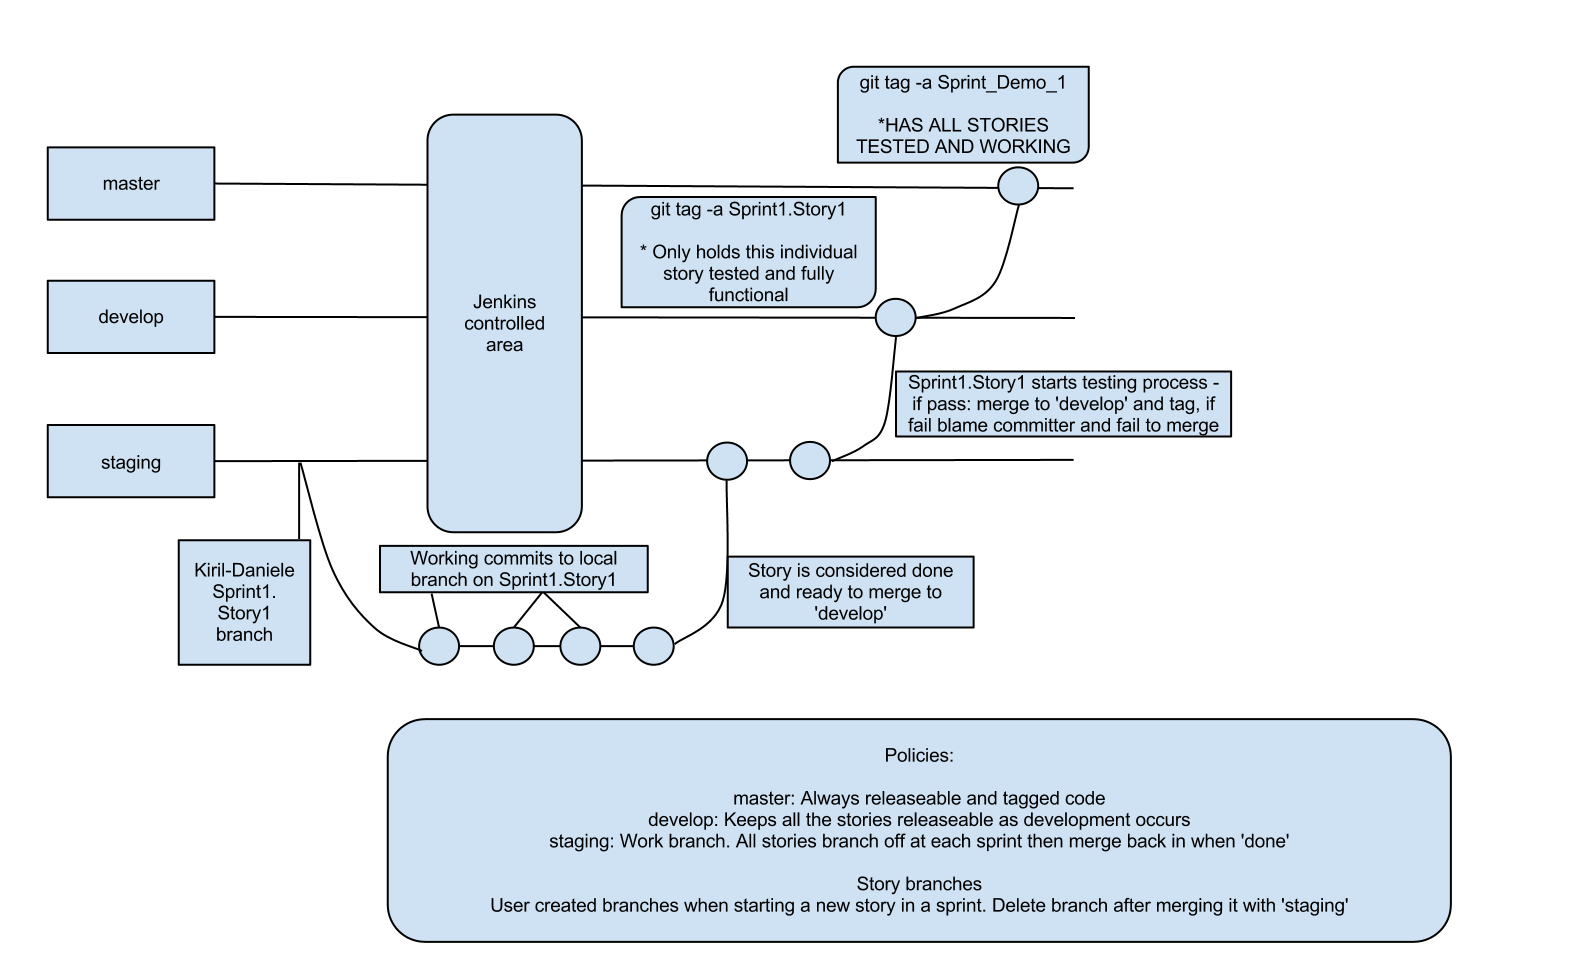
\includegraphics[width=1\textwidth]{img/workflow}
\caption{Sample workflow for one story item}
\label{fig:architecture}
\end{figure}


\subsection{Starting a sprint}

At the start of each sprint the development team will perform a git checkout -b SprintX.shortStoryName DEVELOP

for a running example we will take the HTTP Handler from the first sprint. 
\begin{verbatim}
git checkout -b SprintX.shortStoryName develop
git push -u origin SprintX.shortStoryName
\end{verbatim}
This will pull all the previous items into your temporary working branch from develop

\subsection{Working during a sprint}

As you and your partner work together to complete the tasks outlined in the story, commit as usual to your local branch.\\
\begin{verbatim}
git pull origin staging
git add [files that have been added or created/modified]
git commit -m description - where description is the commit 
message you would like associated with the commit. 
\end{verbatim}
\subsection{Deploying a Done story}

After all the tasks are completed and you feel ready to move the task to the DONE state, merge it to the development branch using the following command:\\

\begin{verbatim}
git checkout staging
git merge --no-ff SprintX.shortStoryName
git push origin staging


- do the following only if you wish to 
delete your branch on the remote repository -
git push origin :SprintX.shortStoryName

- do the following if you wish to delete your branch locally -  
git branch -d SprintX.shortStoryName
\end{verbatim}
This will perform a merge and fast-forward on the remote 'staging' branch while keeping historical information.
This will also create empty commits in the development branch as a way to quickly spot revisions which you may wish to go back to, for example if you need to remove a story that was not working properly.\\\\
%\newpage
\textbf {NOTE:}
As a human user this is typically where you stop working in the workflow. The following steps are to be implemented by Jenkins and automated build tools. You are only concerned with working on the staging branch and your own story branches for each sprint. You should never touch Develop, Master or Release unless absolutey necessary.
%AS A HUMAN USER THIS IS TYPICALLY WHERE YOU STOP WORKING IN THE WORKFLOW. \\THE FOLLOWING STEPS ARE TO BE IMPLEMENTED BY JENKINS AND AUTOMATED BUILD TOOLS. YOU ARE ONLY CONCERNED WITH WORKING ON THE DEVELOP BRANCH AND YOUR OWN STORY BRANCHES FOR EACH SPRINT. YOU SHOULD NEVER TOUCH MASTER OR RELEASE UNLESS ABSOLUTELY NECESSARY

\subsection{Testing a sprint story}

The following steps assume that a testing suite was created and works well with the Jenkins build tool. 

\subsection{Merging in to develop}
When a story branch has been merged to 'staging', the code goes through a set of unit tests and when it successfully passes all of them, it is ready to be merged to 'develop': 
\begin{verbatim}
git checkout develop
git merge --no-ff staging
git push origin develop
\end{verbatim}

\subsection{Merging in to release}
When a story branch has been successfully merged to 'develop', the code goes through a integration test and when it successfully passes it is ready to be merged to 'release': 
\begin{verbatim}
git checkout release
git merge --no-ff develop
git tag -a SprintX.shortStoryName-RELEASE
git push origin release
\end{verbatim}
\subsection{Merging in to master}
Supposing that all the sprint stories code have reached the stage of release, before proceeding with the final merging , we check that all the desired features have been implemented and tested properly.
The final merging is performed upon the MASTER branch containing always the stable version of all the code written so far.
  \begin{verbatim}
git checkout master
git merge --no-ff release
git tag -a Sprint1.Demo1
git push origin master
\end{verbatim}
\subsection{Post-sprint practice}

After each sprint we should synchronize the 'master' and the 'develop' branch. This ensures a clean start for each sprint as the 'staging' branch will inherently be considered the "dirty" branch. 

  \begin{verbatim}
git checkout DEVELOP
git merge --no-ff MASTER
\end{verbatim}

\subsection{References}
The following was an inspiration for the git model:\\

http://nvie.com/posts/a-successful-git-branching-model/
 \\

\chapter{Jenkins Setup}
\label{jenkins-app}
The following guide describes exactly how the ERNI team installed and configured the automated build tool for use during the course. 

\section{Building Jenkins}
Make sure you download the latest *.deb file from the Jenkins website:\\

http://pkg.jenkins-ci.org/debian/\\

To install simply run the following command in a shell:

run Dpkg -; $<$Path\_to\_deb\_file$>$\\

After installed, Jenkins by default starts as a service and runs on port 8080.\\

\section{Jenkins configuration}

Clicking on Configure system  from the Manage Jenkins button will allow you to configure the overall settings of Jenkins. Please note you can also configure *SOME* plugins from here as well. If you do not see the plugin configuration you have installed here, then take a look in the jobs configuration to find settings - if any. 

\subsection {Java JDK}

Before configuring the Java JDK please install it on the server you are working on.
It is required for the Email notification service and also required for Android project building.
\begin{enumerate}
\item Name: $<$enter any name$>$
\item JAVA\_HOME: $<$enter the exact directory on the server machine that holds the bin for jdk $>$ 
\end{enumerate}

\subsection {Android tools}

Before configuring this in Jenkins makes sure you have installed the Android SDK in the server you are working on. 

\begin{enumerate}
\item Enter the path on the server for the Android SDK Root - In our case it is: /home/server-build/android-sdk-linux
\item Check off Automatically install Android components when required
\end{enumerate}
\subsection {Ant}
\begin{enumerate}
\item Enter a Name for the Java ANT environment on the server
\item Check off install automatically.
\end{enumerate}

\subsection{GIT}
Our version of Jenkins requires GIT plugin which can be installed from the manage plugins page.
Scroll down and look for the Jenkins GIT plugin  or use the filter in the top right hand side of the page\\

Setting up the GIT plugin is done from the overall settings page under the section Git plugin.\\

Enter the following settings:
\begin{enumerate}
\item Global Config user.name Value: $<$enter a user name for the git pusher$>$
\item Global Config user.email Value: $<$enter the email for the git pusher$>$
\item Create new accounts base on author/committer's email : checked - this will automatically create people in the Jenkins people page with thier username and email. Also a lookup for the email notifications.
\end{enumerate}
\subsection{JIRA}

Install the JIRA plugin from the manage plugins page. Look for Jenkins JIRA plugin.\\
Setting up the JIRA plugin is done from the overall settings page under the section JIRA.\\
\begin{enumerate}
\item URL:$<$enter the url for the JIRA server$>$
\item Supports Wiki notation: checked
\item Update Jira for All Build Issues: checked
\item User Name: $<$enter the name for the JIRA user bot which will make the updates on JIRA as builds occur
\item Password:$<$enter the password for the JIRA bot$>$
\end{enumerate}


\subsection{Email server}

If you want to have emails being sent from Jenkins the best way is to use the google SMTP server. You will want to set up a project email address at google mail.\\

Enter the following settings in the Email Notification section:
\begin{enumerate}
\item SMTP server: smtp.gmail.com
\item Sender Email-Address: project.cs.2012.uu@gmail.com
\item make sure USE SMTP Authentication is checked.
\end{enumerate}

Click advanced 
\begin{enumerate}
\item Enter the email address name when you set up the account- in our case it is: project.cs.2012.uu@gmail.com
\item Enter the password for the account
\item Check SSL
\item SMTP port set to 465
\item Char-Set is at default: UTF-8
\end{enumerate}

\subsection{Projects}

Jenkins requires Projects in order to do anything useful. \\

To create a new job make sure you are on the jenkins tab, in the top left corner of the webpage. 
Select \textbf{New Job}\\

On the screen 
\begin{enumerate}
\item Enter a Job name - This name will show up on the main dashboard page
\item Select Build a Free-Style software Project.
\end{enumerate}
Click OK when finished and you will be taken to the Configure screen of the project.
Our specific project has the following project properties

(NOTE: steps 14-17 is for erlang only)

\begin{enumerate}
\item Description - enter a project description
\item under Source Code Management Select Git
\item In Repository URL - enter the url for the git repository you will pull from( in our case /home/git/repositories/backend.git)
\item In Branches to build -enter the exact branch you wish to pull and build from. in our case it is origin/BRANCH NAME i.e  origin/STAGING origin/DEVELOP , origin/RELEASE, origin/master. 
\item under Build Triggers Select Poll SCM - enter the time to have jenkins check the git i.e  * * * * * for every minute.
\item under Build click add Build Step and select Execute Shell
\item in the Execute Shell command box - enter any commands required on the commandline in order to build your project. i.e cd netinf\_nrs ; make  etc\ldots
\item under Post-Build Actions click Add post-build action and select Build other projects
\item In Projects to Build - enter the name of the project you wish to start after the selected trigger has been fired.
\item select the trigger Trigger only if build succeeds(used to make sure nothing went wrong with the current project steps).
\item under Post-Build Actions click Add post-build action  and select Email Notification - this action uses the email list built in the people directory in the jenkins main dashboard.
\item check Send e-mail for every unstable build 
\item check Send seperate e-mails to individuals who broke the build 
\item under Post-Build Actions click Add post-build action and select Publish Cobertura Coverage Report	- this will pull erlang eunit and coverage tests into the project main dashboard.
\item In Cobertura xml report pattern - enter  **/*.coverage.xml
\item under Post-Build Actions click Add post-build action and select Publish Junit test Report
\item In Test report XMLs - enter **/.eunit/*.xml

\end{enumerate}

\section {our GIT workflow with Jenkins}

The backend team will use the workflow outlined in the report section Git Workflow. As such the following build projects will be configured for use with Jenkins

\subsection{Backend\_Staging}
\begin{enumerate}
\item Description - "This Job will pull from the Backend Git Repoisitory branch: staging and only check if the source files compile. If they compile then they are passed on to the develop branch."
\item Git Section - URL /home/git/repositories/backend.git
\item Git Section - Advanced - Name: staging
\item Git Section - Branches to build: staging
\item Build Triggers-Poll SCM - * * * * *
\item Build -Execute Shell - cd netinf\_nrs; make compile
\item Post Build Actions - Git Publisher Push only if build succeeds -checked
\item Post Build Actions - Git Publisher Branch to Push: develop
\item Post Build Actions - Git Publisher Target Remote Name: staging
\item Post-Build Actions - Build other projects:  Backend\_Develop
\end{enumerate}
\subsection{Backend\_Develop}

This job assumes all code already compiles when it enters this branch. This branch is specifically for unit tests.

\begin{enumerate}
\item Description -"This job will pull from the Backend Git Repository branch: develop and checks if the source files compile and pass the unit tests. If they compile and pass the tests then they are passed on to the release branch."
\item Git Section - URL /home/git/repositories/backend.git
\item Git Section - Advanced - Name: develop
\item Git Section - Branches to build: develop
\item Build -Execute Shell - cd netinf\_nrs; make compile; make eunit;
\item Post Build Actions - Git Publisher Push only if build succeeds -checked
\item Post Build Actions - Git Publisher Branch to Push: release
\item Post Build Actions - Git Publisher Target Remote Name: develop
\item Post-Build Actions - Build other projects:  Backend\_Release
\end{enumerate}

\subsection{Backend\_Release}

This job assumes all code already compiles AND passes the unit tests. This branch is specifically for integration testing.

\begin{enumerate}
\item Description -"This job will pull from the Backend Git Repository branch: release and checks if the source files compile, pass unit tests and finally pass integration tests. If they compile, and pass all the tests then they are passed on to the master branch(Demo)."
\item Git Section - URL /home/git/repositories/backend.git
\item Git Section - Advanced - Name: release
\item Git Section - Branches to build: release
\item Build -Execute Shell - cd netinf\_nrs; make compile; make eunit; make integration
\end{enumerate}

If the final Backend\_Release succeeds then the following job Backend\_Demo should be taken care of manually until the process is perfected.

\subsection{Backend\_Demo}

This job assumes all code already compiles AND passes the unit tests. This branch is specifically for tagging demos.

\begin{enumerate}
\item Description -"This job will pull from the Backend Git Repository branch: release and checks if the source files compile, pass unit tests and finally pass integration tests. If they compile, and pass all the tests then they are passed on to the master branch(Demo)."
\item Git Section - URL /home/git/repositories/backend.git
\item Git Section - Advanced - Name: release
\item Git Section - Branches to build: release
\item Build -Execute Shell - cd netinf\_nrs; make compile; make eunit; make integration
\item Post Build Actions - Git Publisher Push only if build succeeds -checked
\item Post Build Actions - Git Publisher Add tag - Tag to push: DemoX (where X is the sprint number)
\item Post Build Actions - Git Publisher Target Remote Name: release
\item Post Build Actions - Git Publisher Branch to Push: master
\end{enumerate}

\chapter{Erlang Coding Standards}
\label{erlang-coding-standards}
The purpose of this document is to define coding standards for the NetInf implementation in Erlang. This document is based on the official coding standard and conventions for Erlang (http://www.erlang.se/doc/programming\_rules.shtml\#REF87730). 

\section{Engineering Principles}
\subsection{Export As Few Functions As Possible From a Module}
For better readability and understanding of code it is recommended that we export as few functions as possible. When exporting a function you should define specification (a.k.a contract) with the erlang “-spec” compiler attribute (http://www.erlang.org/doc/reference\_manual/typespec.html\#id75681). 

\subsection{Prefer Readability Over Speed}
It is recommended that we initially write code that is easy to read instead of writing code that makes the program run fast but hard to understand. However if run time complexity becomes a problem, consider rewriting the code in an optimized way. 

\subsection{Directory Structure of an OTP Application}
Erlang/OTP applications should have a directory structure as shown below:
\begin{lstlisting}	
<application-name> [-<version>]
                   |
                   |-doc
                   |-ebin
                   |-include
                   |-priv
                   |-src
\end{lstlisting}
Where: 
\begin{description}
\item[doc] This is where you put your overview.edoc file if you generate documentation from EDoc. 
\item[ebin] This is where your compiled code (.beam files) and meta data file (.app) is located. 
include: Your public header files (.hrl file) should be kept in this directory.  
\item[priv] Here you should put template files, shared objects and DLLs. 
\item[src] This should have source code related to your application which includes .erl files and internal .hrl files. It can also have ASN.1, YECC, MIB and other source files.
\end{description}

\section{Specific Lexical and Stylistic Conventions}
Use Emacs and Erlang mode when writing code. To get to correct indentation just press ‘Tab’ when you are in Erlang mode. We recommend that everyone use Emacs for writing the code because this way everybody in the team will be familiar with everyone else’s development environment. This is important in case we decide to do pair programming. 

\begin{itemize}

\item Don’t write deeply nested code which means not more than 2 levels of indentation. 
\item Don’t write larger modules than 400 lines. 
\item Don’t write long lines, at most 78 characters.
\item Don’t write longer functions than 15 to 20 lines. 
\item Choose meaningful variable names and use capitalized letter to separate the words. Example: ReceivedMessage
\item The function name should represent what the function does. Use underscore to separate different words. Example: send\_message().
\item Give space after each argument in a data structure or function arguments. Example {12, 13, 45}.
\item Use tagged return values. This means that the return value of the functions should be a tuple where the first key should be an atom explaining what it is.  
\item Don't use -import
\item Use multiple -export clauses instead of grouping a lot of functions together in one export clause. Examples:  user interface, intermodule exports and exports for use within module only. 
\item Always use proper indentation.
\item Do not comment out old code, just remove it because it is already in the source control repository.  
\end{itemize}
  
\subsection{Comments and Documentation}
Instead of littering your code with comments you should write meaningful variable and function names. But in some cases where the code is hard to understand you can write short comments. For every function use Edoc notation and explain arguments and return value and if present, side effects. (http://www.erlang.org/doc/apps/edoc/chapter.html).  

Each file should start with a short description of the module contained in the file and a brief description of all exported functions. All the error messages in an application should be documented in a single document.  





\chapter{Java and Android Coding Standards}
\label{java-coding-standards}
\lstset{language=Java}

The purpose of this section is to present the code convention used in the implementation of the Android-based application. These code standards are based
on the Android Code Style Guidelines for Contributors\footnote{\url{http://source.android.com/source/code-style.html}}.

\section{Java Language Rules}

\begin{itemize}
  \item Do not ignore exceptions. It is only acceptable to ignore exceptions if there is a good reason to do it, which should be given as a comment in the code. As a general rule, always:
  \begin{itemize}
   \item handle the exception;
   \item or throw a new exception according to the level of abstraction;
   \item or handle it gracefully;
   \item or throw a new \textit{RuntimeException} in case there is nothing possible to do.
  \end{itemize}
  \item Don't catch a generic exception e.g. \textit{Exception e}. Alternatives to do this are:
 \begin{itemize}
    \item Catch each exception with a separate catch block after a single try.
    \item Refactor the code in order to have muliple try blocks.
    \item Rethrow the exception and let it be handle in the next level.
  \end{itemize}
  \item Do not use finalizers. Let the garbage collector do its job
  \item Always write full imports.
  
  \section{Java Style Rules}
  \item Use Javadoc standards for commenting code. Always write the descriptions in third person. This rule can be skipped if the method is too trivial e.g. a \textit{getters} and \textit{setters}.
  \item Try not to exceed 40 (forty) lines of code for each method.
  \item Try to keep the scope of a variable as small as possible. Also, try to initialize it with a proper value. 
  \item Order the imports beginning with Android libraries, followed by third parties libraries and ending with \textit{java} and \textit{javax} classes, each group separated by an empty line.
  \item For identation, use four spaces for blocks and eight spaces for line wraps (i.e. when the line of code is too long and needs to be cut).
  \item Limit the line length to 80 (eighty) characters. 
  \item Use standard Java Annotations e.g. \textit{@Deprecated, @Override, @SuppressWarnings}.
  \item Use acronyms as words e.g. write \textit{XmlHttpRequest} not \textit{XMLHTTPRequest}.
  \item Use TODO comments for temporary fixes and future work.
  \item Use all five levels of logging (Error, Warning, Informative, Debug and Verbose) as applicable.
  \item Use the standard brace style: 
  \begin{lstlisting}
      public void foo() {
	  if (...) {
	      doSomething();
	  }
      }
  \end{lstlisting}
  \item Use the following naming conventions:
  \begin{itemize}
    \item Non-public, non-static field names start with m.
    \item Static field names start with s.
    \item Other fields start with a lower case letter.
    \item Public static final fields (constants) are letters in upper case and spaces replaced by underscores.
    Example:
      \begin{lstlisting}
      public class MyClass {
	  public static final int SOME_CONSTANT = 42;
	  public int publicField;
	  private static MyClass sSingleton;
	  int mPackagePrivate;
	  private int mPrivate;
	  protected int mProtected;
      }
      \end{lstlisting}
    \end{itemize}
  \end{itemize}

\bibliography{references}
\bibliographystyle{plain}

\end{document}
